\NeedsTeXFormat{LaTeX2e}
\documentclass[a4paper,12pt,
headsepline,           % Linie zw. Kopfzeile und Text
oneside,               % einseitig
pointlessnumbers,      % keine Punkte nach den letzten Ziffern in Überschriften
bibtotoc,              % LV im IV
%DIV=15,               % Satzspiegel auf 15er Raster, schmalere Ränder   
BCOR15mm               % Bindekorrektur
%,draft
]{scrbook}
\KOMAoptions{DIV=last} % Neuberechnung Satzspiegel nach Laden von Paket helvet

\pagestyle{headings}
\usepackage{blindtext}

% für Texte in deutscher Sprache
%\usepackagemngerman]{babel}
\usepackage[utf8]{inputenc}
\usepackage[T1]{fontenc}

% Helvetica als Standard-Dokumentschrift
\usepackage[scaled]{helvet}
\renewcommand{\familydefault}{\sfdefault} 

\usepackage{graphicx}

% Literaturverzeichnis mit BibLKaTeX
\usepackage[babel]{csquotes}
\usepackage[backend=biber]{biblatex}
\bibliography{bibliography}
\AtEveryBibitem{%
  \clearfield{note}%
}

\usepackage{tabularx} 

% Besondere Schriftauszeichnungen
\usepackage{url}              % \url{http://...} in Schreibmaschinenschrift
\usepackage{color}            % zum Setzen farbigen Textes

\usepackage{amssymb, amsmath} % Pakete für Mathe-Umgebungen und -Symbole

\usepackage{setspace}         % Paket für div. Abstände, z.B. ZA
\usepackage{subcaption}
%\onehalfspacing              % nur dann, wenn gefordert; ist sehr groß!!
\setlength{\parindent}{0pt}   % kein linker Einzug der ersten Absatzzeile
\setlength{\parskip}{1.4ex plus 0.35ex minus 0.3ex} % Absatzabstand, leicht variabel

\usepackage{todonotes}
\usepackage{algorithm}
\usepackage[noend]{algpseudocode}
\usepackage{diagbox}
\usepackage{booktabs}
\usepackage{siunitx}

\makeatletter
\def\BState{\State\hskip-\ALG@thistlm}
\makeatother

% Tiefe, bis zu der Überschriften in das Inhaltsverzeichnis kommen
\setcounter{tocdepth}{3}      % ist Standard

\newcommand{\fullname}{Paul Nykiel}
\newcommand{\email}{paul.nykiel@uni-ulm.de}
\newcommand{\titel}{Fast Object Detection in Dense Pointclouds}
\newcommand{\jahr}{2019}
\newcommand{\matnr}{941496}
\newcommand{\gutachterA}{Prof. Dr.-Ing. Klaus Dietmayer}
\newcommand{\gutachterB}{Jun.-Prof. Dr. rer. nat. Vasileios Belagiannis  }
\newcommand{\betreuer}{Martin Herrmann}

\newcommand{\fakultaet}{Ingenieurwissenschaften, Informatik und\\Psychologie}
\newcommand{\institut}{Institut für Mess-, Regel- und Mikrotechnik}

% Informationen, die LaTeX in die PDF-Datei schreibt
\pdfinfo{
  /Author (\fullname)
  /Title (\titel)
  /Producer     (pdfeTex 3.14159-1.30.6-2.2)
  /Keywords ()
}

\usepackage{hyperref}
\hypersetup{
pdftitle=\titel,
pdfauthor=\fullname,
pdfsubject={Diplomarbeit},
pdfproducer={pdfeTex 3.14159-1.30.6-2.2},
colorlinks=false,
pdfborder=0 0 0	% keine Box um die Links!
}

% Trennungsregeln
\hyphenation{Sil-ben-trenn-ung}

\begin{document}
\frontmatter

% Titelseite
\thispagestyle{empty}
\begin{addmargin*}[4mm]{-10mm}


\includegraphics[height=1.8cm]{images/unilogo_bild}
\hfill

\includegraphics[height=1.8cm]{images/unilogo_wort}\\[1em]

{\footnotesize
%{\bfseries Universität Ulm} \textbar ~89069 Ulm \textbar ~Germany
\hspace*{115mm}\parbox[t]{35mm}{\bfseries Fakultät für\\
\fakultaet\\
% TODO hier Institut anpassen
\mdseries \institut}\\[2cm]

\parbox{140mm}{\bfseries \LARGE \titel}\\[2.5em]
{\footnotesize Abschlussarbeit an der Universität Ulm}\\[3em]

{\footnotesize \bfseries Vorgelegt von:}\\
{\footnotesize \fullname\\ \email}\\ \matnr\\[2em]
{\footnotesize \bfseries Gutachter:}\\                     
{\footnotesize \gutachterA\\ \gutachterB}\\[2em]
{\footnotesize \bfseries Betreuer:}\\ 
{\footnotesize \betreuer}\\\\
{\footnotesize \jahr}
}
\end{addmargin*}


% Impressum
\clearpage
\thispagestyle{empty}
{ \small
  \flushleft
  Version \today \\\vfill
  \copyright~\jahr~\fullname\\[0.5em]
% Wenn Sie Ihre Arbeit unter einer freien Lizenz bereitstellen möchten, können Sie die nächste Zeile in Ihren Code aufnehmen. Bitte beachten Sie, dass Sie hierfür an allen Inhalten, inklusive enthaltener Abbildungen, die notwendigen Rechte benötigen! Beim Veröffentlichungsexemplar Ihrer Dissertation achten Sie bitte darauf, dass der Lizenztext nicht den Angaben in den Metadaten der genutzten Publikationsplattform widerspricht. Nähere Information zu den Creative Commons Lizenzen erhalten Sie hier: https://creativecommons.org/licenses/
This work is licensed under the Creative Commons Attribution 4.0 International (CC BY 4.0) License. To view a copy of this license, visit \href{https://creativecommons.org/licenses/by/4.0/}{https://creativecommons.org/licenses/by/4.0/} or send a letter to Creative Commons, 543 Howard Street, 5th Floor, San Francisco, California, 94105, USA. \\
  Satz: PDF-\LaTeXe
}

% ab hier Zeilenabstand etwas größer 
\setstretch{1.2}

\tableofcontents

\mainmatter
\chapter{Introduction}

In recent years many improvements in driver assistance systems have been made \cite{autonomesFahren}.
Vehicle manufactures and researchers aim to produce fully self driving vehicles in the next years.
Such vehicles are able to drive according to the traffic rules without human involvement.
For this a wide variety of algorithms have to be developed, implemented and tested.
These algorithms need to be reliable to guarantee the safety of the passengers and all other road users. Additionally the algorithms are required to process the sensor data in real time to guarantee a timely response of the vehicle.

To get students interested in the topic of self driving systems and driver assistance systems the University of Technology Braunschweig organizes the Carolo-Cup. The aim of the competition is
to build an automated \ac{rc}-Car at a scale of 1:10. 
The vehicle needs to master a scenario which is derived from scenarios that occur in the real world and drive as far as possible. 
The scenario consists of the track with road markings, crossings, obstacles, signs, pedestrians and slopes. Each of these features need to be detected by the vehicle in real time.

Ulm University is participating in this competition with a group of students. The primary sensors of the vehicle are a colour camera and an \ac{d435} which captures a point cloud.

The objective of this work is to implement an algorithm which is able to robustly detect and classify all objects occurring on the track, that are signs, obstacles, pedestrians and slopes, using the point cloud provided by the \ac{d435}. 
The algorithm used for the detection should be able to process the data in real time with the limited resources available on the vehicle to be able to be used on the vehicle.

Additionally the algorithm should be evaluated on point clouds acquired in the real world using a stereo camera system. For this data from the MEC-View project \cite{mec} and the Kitti dataset \cite{Menze2015CVPR} is used.

The thesis is structured in four chapters:
in Chapter \ref{sec:theo} the theoretical background required for the thesis is explained. Chapter \ref{sec:det} introduces the algorithm used for object detection. In Chapter \ref{sec:eval} the performance of the algorithm is evaluated and compared to other algorithms. Lastly the results are summarized and possible future improvements are listed in Chapter \ref{sec:conc}.


\chapter{Theoretical Background} \label{sec:theo}
This chapter will introduce the fundamentals necessary to understand the following chapters. The first section will define the coordinate systems used in this thesis.
Next point clouds are introduced  and algorithms and sensors for generating them are presented.
The following section will present an efficient connected components labeling algorithm.
The next section explains artificial neural networks and \acp{cnn}.
In the last section the \ac{pca} is introduced.

\section{Coordinate Systems} 
\subsection{Vehicle Coordinate System} \label{sec:theo:vehicleCoord}
According to ISO 8855 \cite{ISO8855} 
a vehicle axis system is defined with the $x$-axis pointing horizontally forward. 
The $y$-axis is horizontal as well, pointing left with respect to the forward direction. The $z$-axis points upwards, so that it forms a right handed trihedron. The rotation around the $x$-axis is referred to as roll, the rotation around the $y$-axis as pitch and the rotation around the $z$-axis as yaw or heading.
The vehicle coordinate system is defined by the vehicle axis system and the vehicle reference point, that is the origin of the coordinate system.

If not stated otherwise this work will use this coordinate system with the vehicle reference point located in the centre of the camera.

\begin{figure}[h!]
    \centering
    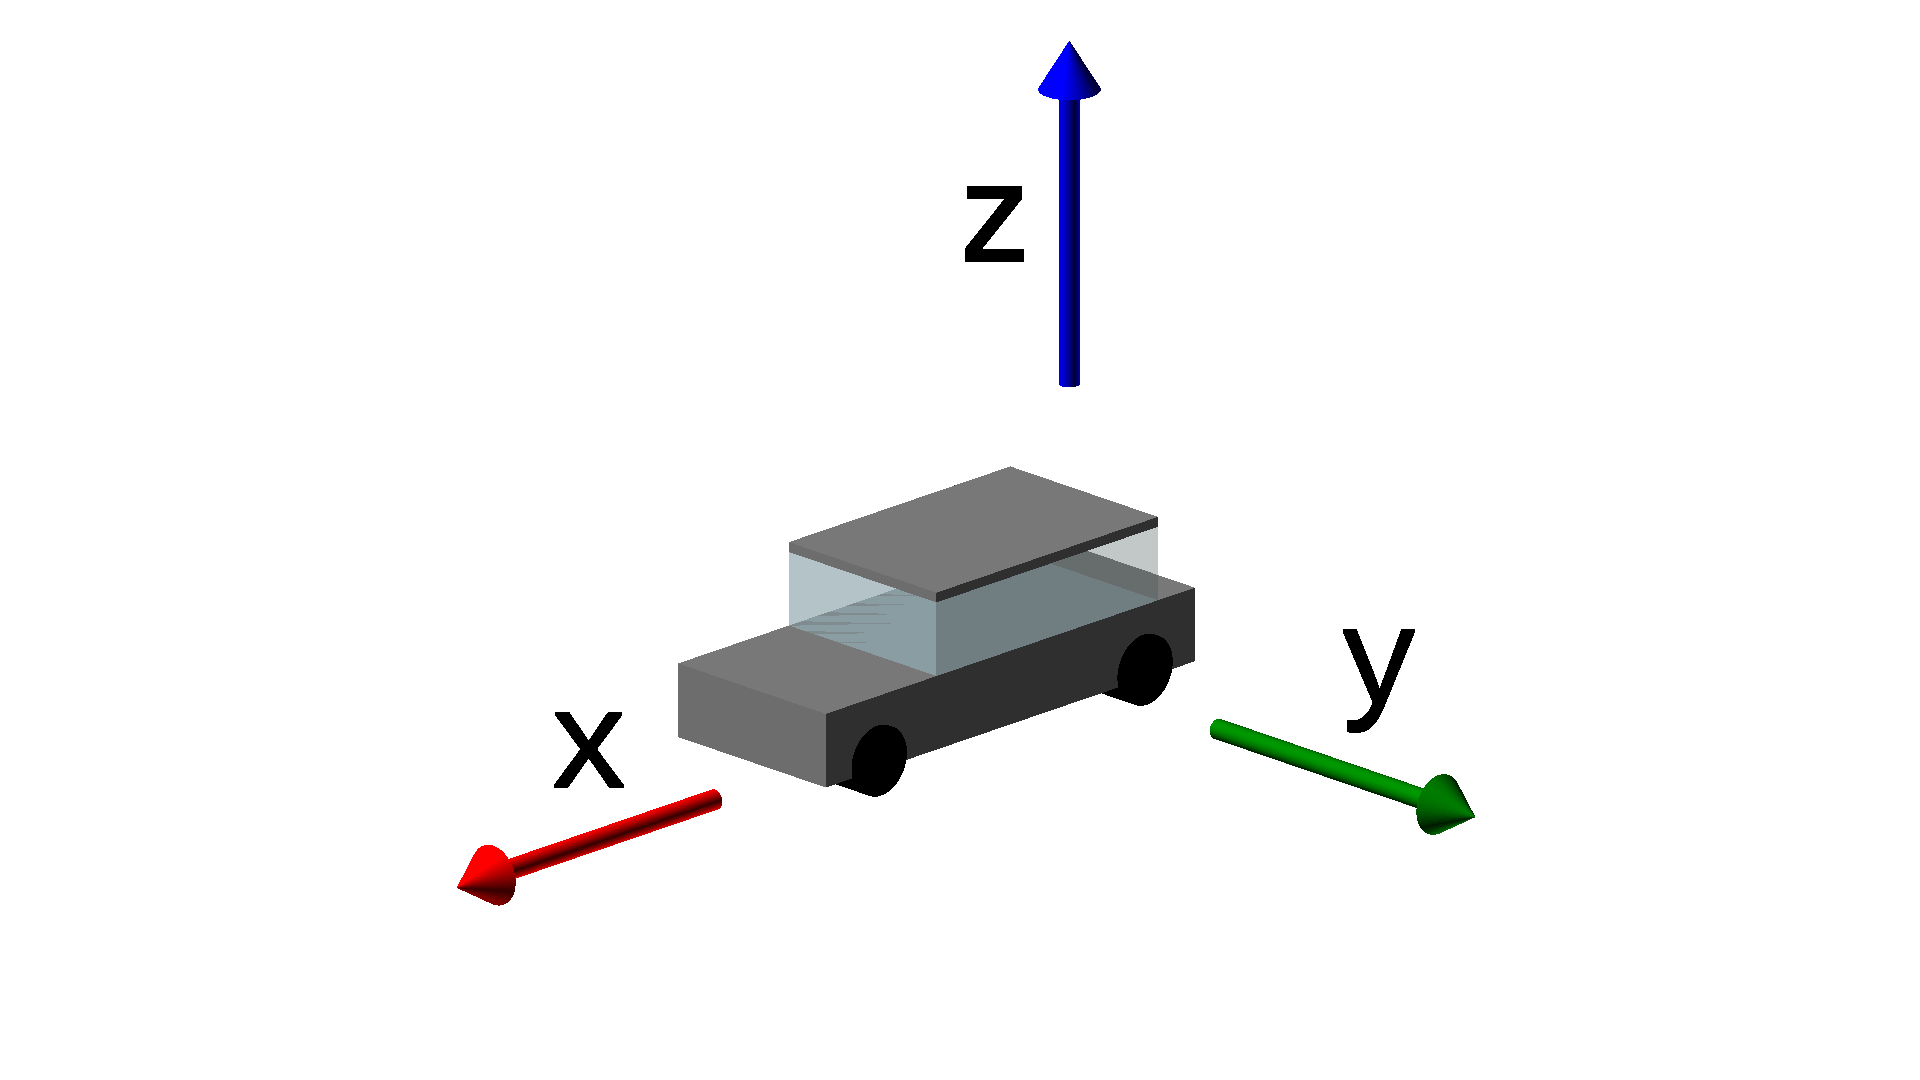
\includegraphics[width=\textwidth]{coord.png}
    \caption{Vehicle Coordinate System (Source: Own illustration)}
    \label{fig:theo:coord}
\end{figure}

\subsection{Image Coordinate System} \label{sec:theo:imageCoord}
For images the coordinate system consists of a $x$-axis pointing right and a $y$-axis pointing downward. The origin of the coordinate system is in the top left of the image.

\begin{figure}[h!]
    \centering
    \begin{tikzpicture}[scale=0.5]
        \pgfmathtruncatemacro{\scale}{1}
        \foreach \x in {0,1,...,9}{
            \foreach \y in {0,1,...,9}{
                \pgfmathtruncatemacro{\xpos}{\x * \scale};
                \pgfmathtruncatemacro{\ypos}{\y * \scale};
                \filldraw [draw=black,fill=gray!40] (\xpos,\ypos) rectangle (\xpos+\scale,\ypos+\scale);
            }
        }
        \draw[line width=3pt,arrows={-triangle 60}] (-1,10) -- (-1,0);
        \node (y) at (-2,5){$y$}; 
        \draw[line width=3pt,arrows={-triangle 60}] (0,11) -- (10,11);
        \node (x) at (5,12){$x$}; 
        
    \end{tikzpicture}
    \caption{Image Coordinate System (Source: Own illustration)}
\end{figure}

\section{Point Clouds}
A point cloud is a set of points in space, that is usually the $\mathbb{R}^3$. A point cloud is either created artificially or more commonly captured by a sensor, in
this case the point cloud gets sampled from a 3D object \cite{pclAbout}.

\begin{figure}[h!]
    \centering
    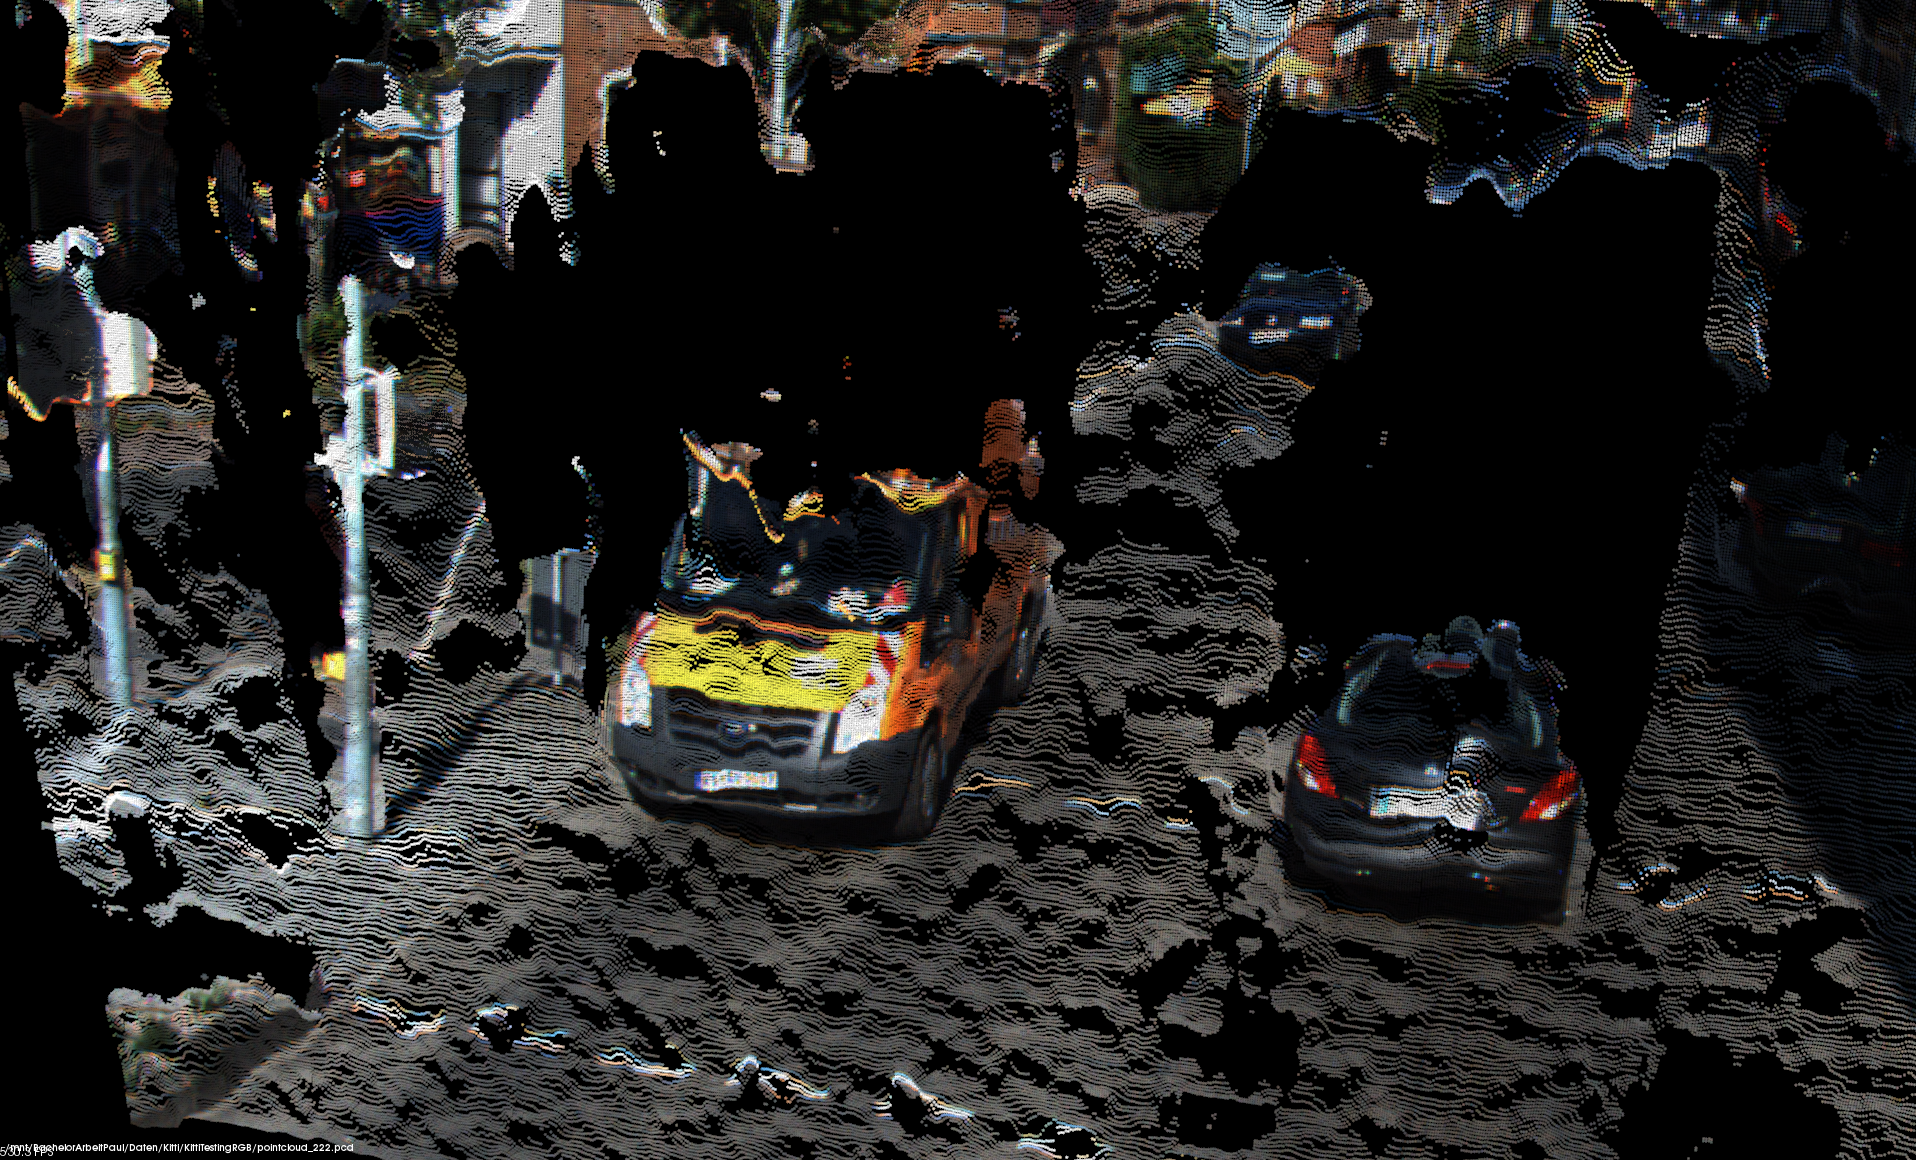
\includegraphics[width=\textwidth]{../Material/pointcloud.png}
    \caption{Example of a point cloud with additional colour information}
    \label{fig:theo:pc}
\end{figure}

Each point in a point cloud is usually represented by a vector consisting of the $x$, $y$ and $z$ coordinate. In addition to the coordinates more information can be stored for every point. Commonly used values are the reflectivity, surface normals or the colour of each point. 

Figure \ref{fig:theo:pc} shows a point cloud which depicts an urban scene,
the point cloud is generated from the Kitti dataset \cite{Menze2015CVPR}.
In addition to the points in space there is also colour information for every point.
This additional colour information is often referred to as texture \cite{pclAbout}.

\subsection{Stereo Vision}
By taking pictures from a scene from two positions it is possible to calculate distance information from the scene by exploiting the difference between the images \cite{stereoHaw10}.
This process is called stereo vision and is similar to what the human brain does with the information of two eyes. 

In general, stereo vision is based on matching a pixel found in one of the images to a pixel in the second image. 
The distance between the two positions of the pixels is called disparity, which is inverse proportional to the actual distance of the point. 
By combining the disparity for every pixel into an image at the corresponding position a disparity image or disparity map is created.

\begin{figure}[h!]
    \centering
    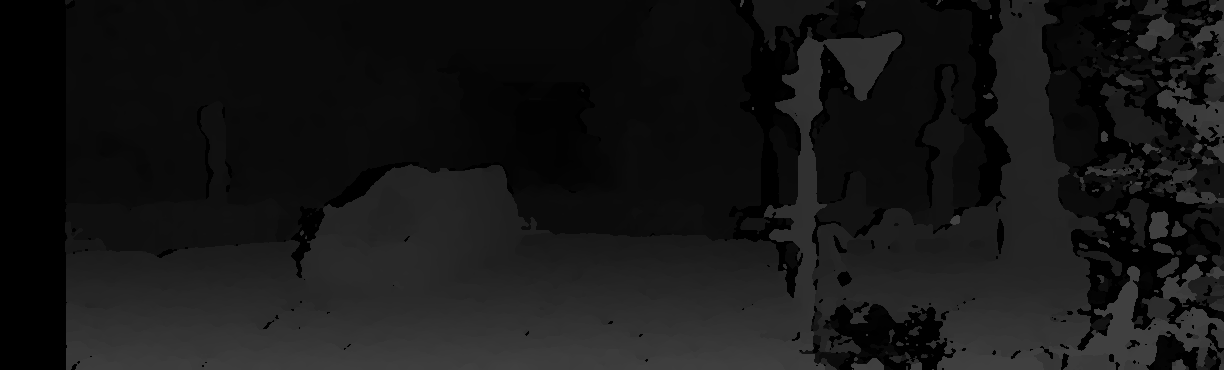
\includegraphics[width=\textwidth]{disparity.png}
    \caption{Example of a disparity map }
    \label{fig:theo:disp}
\end{figure}

Figure \ref{fig:theo:disp} shows a disparity map generated from the Kitti dataset \cite{Menze2015CVPR}, the disparity values are mapped onto different colours, with orange being large disparities and blue small disparities.

In the following sections two algorithms for the calculation of disparity maps are presented.

\subsubsection{Rectification}
For a pixel in one of the images all possible points in the real world are located on a line \cite{stereoHaw10}.
In the second image this set of points is visible as a line, which is called the epipolar line. 
As all pixels that can possible correspond to a pixel in the first image lie on the epipolar line on the second image it is sufficient to only search for matches on this line.
To simplify the matching it is beneficial for the epipolar line to be straight and horizontal.
This is achieved by rectifying the image, that is transforming the images, such that all epipolar lines are horizontal. This results in transformed images which appear to be taken with two cameras with only horizontal displacement and no relative rotation.

\begin{figure}[h!]
    \centering
    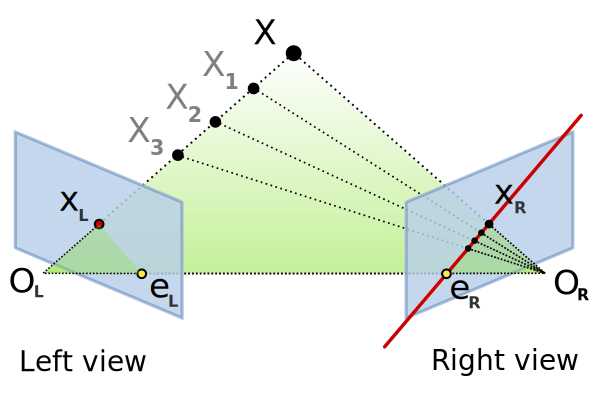
\includegraphics[width=\textwidth]{EpipolarGeometry.pdf}
    \caption{Point as part of the epipolar line (Source: Arne Nordmann [cc by-sa 3.0])}
    \label{fig:theo:epipolarLine}
\end{figure}

Figure \ref{fig:theo:epipolarLine} shows the views of a stereo system with the left camera, positioned at $O_L$, and the right camera positioned at $O_R$. 
All points $X$, $X_1$, $X_2$ and $X_3$ are located on a straight line and are projected to the same pixel $X_L$ in the left image. 
In the right image the points are located on a straight line, this line can be seen as the red line. 
All possible matches $X_R$ for the pixel $X_L$ are located on this epipolar line.
As the epipolar line is not horizontal the images require rectification.

Rectification is done by linear transforming the images. For this a transformation matrix $H$, so that an image point $p$ is transformed into $\vec{p}$ need to found.

\subsubsection{Semi-Global Matching} \label{sec:theo:sgm}
Semi-Global Matching \cite{Hirsch05} \cite{sgm2} is one the most commonly used \cite{stereoHaw10} algorithms for calculating disparity maps, primarily based on the fact that it is able to run in real time  while still producing precise results \cite{middleburyStereo3}. 
The algorithm performs dense stereo matching, this implies that for nearly every pixel a corresponding pixel is found. 
The algorithm combines the advantages in computational performance of pixel wise matching with the advantages in quality of a global cost function, which considers the complete image for matching.

The global cost function is accumulated over eight directions: both vertical directions, and horizontal directions and the diagonal directions. For every direction the cost function is calculated independently.

The cost function is calculated by scanning the image along the respective directions. 
This reduces the problem from a two dimensional problem to multiple one dimensional problems on a scanline \cite{sgmHeidelberg}.

Along this scanline a similarity function $C: (p,d) \to \mathbb{R}$ is calculated. This function represents the similarity of a pixel $p$ to a pixel $\tilde{p}$ with disparity $d$. 
This similarity can be calculated by comparing the intensity at the position $p$ with the intensity at the pixel $\tilde{p}$.
This second pixel is the pixel on the epipolar line with a distance of $d$ from $p$.
The algorithm selects a disparity for every pixel. As the pixels next to each other are not independent of each other the similarity of the disparity, that is the smoothness of the resulting disparity map, should be enforced. 
For this a loss function $L_\text{Direction}(p,d)$ considering the neighbouring pixels is defined, using the constants $P_1$ and $P_2$ as non smoothness penalty:
\begin{eqnarray}
    n_i &=& L_\text{Direction}(p-1,d+i) \\
    L_\text{Direction}(p,d) &=& C(p,d) + \min\{n_0, n_1 + P_1, n_{-1} + P_1, \min_i (n_i) + P_2\}
\end{eqnarray}
The loss is calculated twice along the scanline, first in a forward pass and secondly backwards along the scanline. For every pixel a loss over all directions is calculated as the sum of the losses in the different directions:
\begin{equation}
    L_\text{Overall}(p,d) = \sum_{\text{Direction} \in \text{All Directions}} L_\text{Direction}(p,d)
\end{equation}

Using the overall loss for every pixel the disparity $d$ for a pixel $p$ can now be calculated as the disparity with the lowest loss, to speed up the computation a maximum disparity $d_\text{max}$ is used:
\begin{equation}
    d(p) = \text{argmin}_{d \in \{0, \ldots, d_\text{max} \} } \left(L_\text{Overall}(p,d)\right)
\end{equation}

% https://www.reddit.com/r/computervision/comments/9119qc/can_i_have_a_pseudo_code_explanation_of_the/

%http://lunokhod.org/?p=1356

\subsubsection{Calculating point clouds from Disparity Maps} \label{sec:theor:disp2pc}
Given the parameters of the individual cameras such as the focal length, and the parameters of the stereo system such as the translation and rotation between the two vantage points it is possible to compute the real world distances and as a result positions of pixels relative to the camera \cite{opencvpc}. 
Taking all these pixels as points in three dimensional space a point cloud can be calculated.
By additionally mapping the colour of each pixel onto the corresponding point a texture for the point cloud can be calculated.

Given the disparity $d(x,y)$ at a pixel ${(x,y)}^\text{T}$ and the corresponding calibration matrix $Q$ for the stereo system the position of the point in 3D space can be calculated:
\begin{eqnarray}
    \begin{pmatrix} 
        X \\ Y \\ Z \\ W
    \end{pmatrix}
    &=& Q \cdot 
    \begin{pmatrix}
        x \\ y \\ d(x,y) \\ 1
    \end{pmatrix} \\
    \vec{p}_\text{real world} &=& 
    \frac{1}{W}
    \begin{pmatrix}
        X \\ Y \\ Z
    \end{pmatrix}
\end{eqnarray}

\subsubsection{Depth Error Estimate} \label{sec:theo:error}
For many applications it is desirable to estimate the error of the depth measurement of a stereo system.
The depth error can be estimated given the distance $d$ to the object, the baseline $b$ that is the distance between the cameras, the focal length $f$ of the cameras and pixel matching error $\varepsilon_d$ \cite{stereoError}:
\begin{equation}
    \varepsilon \propto \frac{d^2}{b\cdot f} \cdot \varepsilon_d
\end{equation}

\subsection{Active Stereo Systems}
Passive vision based stereo systems have issues with textureless surfaces as no unambiguous correspondences can be found \cite{d435Structured}.
Additionally passive vision systems perform poor matching if the scene is not illuminated well.
To solve both issues an active system can be used. 
These systems use a projector to project an pattern onto the surface and thus provide a texture for every surface.
No a priori knowledge of the pattern or adaptation of the stereo matching algorithm is required \cite{d435Structured}.
To achieve unambiguous matches a non periodic pattern should be chosen, this can be done by using a semi-random pattern.

The \ac{d435} uses a projector which projects about 5000 points in a semi-random fashion using a laser projector \cite{d435Structured}.

%https://www.intelrealsense.com/wp-content/uploads/2019/03/WhitePaper\_on\_Projectors\_for\_RealSense\_D4xx\_1.0.pdf}
%https://www.intelrealsense.com/stereo-depth-vision-basics/}

\section{Connected Components Labeling} \label{sec:theo:concomp} 
Connected components labeling is used to find connected nodes in a graph.
Two nodes $n$ and $m$ of the same class are connected if there exists a path between them consisting entirely of nodes of their class \cite{digitalImageProcessing}.
The algorithm takes the graph as the input and returns for every class a set of nodes that belong to the class.

The algorithms for connected components labeling can be differentiated in one component at a time algorithms, which label objects separately \cite{abubaker2007}, and multipass algorithms which iterates over the nodes multiple times \cite{HeChaoSuzuki08}.

\cite{HeChaoSuzuki08} proposed an efficient two pass algorithm for connected components labeling.
The algorithm is designed to be used with images.
For images every pixel represents a node in the graph. 
The eight adjacent pixels of a pixel are the neighbouring nodes.
As the number of neighbours is bounded the algorithm runs in $\mathcal{O}(n)$ with $n$ being the number of pixels. 

The algorithm is explained in algorithm \ref{alg:theo:concomp}: first for every pixel a preliminary class is determined based on the neighbouring pixels, additionally equivalent classes are remembered. 
In the second step all identical classes are merged into the class with the lowest number.

% See: https://scicomp.stackexchange.com/questions/1429/dictionaries-in-pseudocode for dict
\begin{algorithm}[h!]
    \caption{Connected Components Labeling}\label{alg:theo:concomp}
    \begin{algorithmic}[1]
        \Procedure{ConnectedComponentsLabeling}{nodes}
            \State $\text{class} \gets -1 \text{ for every node} \in \text{nodes}$
            \State $\text{currClass} \gets 0$
            \State $\text{mappingToMinimal} \gets \text{empty dictionary}$
            \For {node $\in$ nodes} 
            \Comment{First pass: label all by neighbours, remember equivalent classes}
                \State equivalentClasses $\gets \emptyset$
                \For {neighbour $\in$ neighbours of node}
                    \If {$\text{sameClass}(\text{node}, \text{neighbour}) \land \text{class}[\text{neighbour}] >= 0$}
                        \State equivalentClasses $\gets \text{equivalentClasses} \cup \{\text{class}[\text{neighbour}]\}$
                    \EndIf
                \EndFor

                \If {equivalentClasses $= \emptyset$}
                    \State $\text{currClass} \gets \text{currClass} + 1$
                    \State $\text{class}[\text{node}] \gets \text{currClass}$
                \Else
                    \State $\text{minClass} = \gets \min(\text{equivalentClasses}$
                    \For {$\text{class} \in \text{equivalentClasses} \setminus \{\text{minClass}\}$}
                        \State $\text{mappingToMinimal}[\text{class}] = \text{minClass}$
                    \EndFor
                \EndIf
            \EndFor

            \For {node $\in$ nodes}
            \Comment{Second pass: merge equivalent classes}
                \While {$\text{class}[\text{node}] \in \text{mappingToMinimal}$}
                    \State $\text{class}[\text{node}] \gets \text{mappingToMinimal}[\text{class}[\text{node}]]$
                \EndWhile
            \EndFor
        \EndProcedure
    \end{algorithmic}
\end{algorithm}


\section{Artificial Neural Networks}
Artificial Neural Networks are algorithms, that mimic the human brain \cite{Hodgkin1952}. They consist of a set of neurons connected together as a graph. Each neuron takes a number of inputs, combines them with a given formula and produces an output, which is then propagated to the next neuron.
The parameters of the formula can be changed to adapt the output of the neural network.

For most neural networks there are two main phases \cite{bishop1995}: first learning, that is adapting the parameters to fit a certain function and forwarding, that is calculating the output for data the neural networks has not seen before.

There are three different paradigms for learning: unsupervised learning, which is used for tasks such as feature extraction and clustering, reinforcement learning, which is used if a reward can be defined but no ground truth data exists, and supervised learning which is used if labeled ground truth data exists. As this is the case for the neural network used in this thesis, only supervised learning will be explained in the following section.

In the following section first a simple neural network, the \ac{mlp} is explained.
Then the \acf{cnn} is explained as a special case of a \ac{mlp}.

\subsection{Neuron}
\cite{Hodgkin1952} modeled the activity of a neuron in the human brain with a continuous differential equation.
For larger neural networks this differential equation gets to complicated.
Thus the model has been simplified \cite{bishop1995}: The output is determined by calculating the weighted sum of all inputs $x_k$ and adding a so called bias $b$.
To be able to approximate nonlinear functions a nonlinear transfer function $f$ is then applied for every neuron:

\begin{equation}
    y = f\left(b + \sum_{k=1}^n x_k \cdot w_k \right)
\end{equation}

The structure of a neuron can be seen in Figure \ref{fig:theo:neuron}, the inputs $x_1$ to $x_n$ are on the left side of the neuron. Each of the input values is weighted and the values are then summed up in the neurons. Lastly the transfer function is applied, the output value $y$ is at the right side of the neuron.

\begin{figure}[h!]
    \centering
    \begin{tikzpicture}[scale=.7]
        \pgfmathtruncatemacro{\x}{4};

        \draw (0,0) -- (-\x,{\x*sin(60)});
        \node[anchor=east] at (-\x,{\x*sin(60)}) (x1) {$x_1$};
        \node[anchor=south] at ({-\x*3/4},{\x*3/4*sin(60)}) (w1) {$w_1$};

        \draw (0,0) -- (-\x,{\x*sin(30)});
        \node[anchor=east] at (-\x,{\x*sin(30)}) (x2) {$x_2$};
        \node[anchor=south] at ({-\x*3/4},{\x*3/4*sin(15)}) (w2) {$w_2$};

        \node[anchor=east] at (-\x,{-\x*sin(0)}) (vdots) {$\vdots$};

        \draw (0,0) -- (-\x,{-\x*sin(30)});
        \node[anchor=east] at (-\x,{-\x*sin(30)}) (xn) {$x_n$};
        \node[anchor=south] at ({-\x*3/4},{-\x*3/4*sin(30)}) (wn) {$w_n$};

        \draw (0,0) -- (-\x,{-\x*sin(60)});
        \node[anchor=east] at (-\x,{-\x*sin(60)}) (b) {$b$};

        \draw (0,0) -- (\x,0) node[anchor=west] (y) {$y$};

        \filldraw[fill=primary] (0,0) circle (2);
        \node at (-1,0) (sum) {\scalebox{2}{$\sum$}};
        \draw (0,2) -- (0,-2);
        \node at (1,0) (f) {\scalebox{2}{$f$}};
    \end{tikzpicture}
    \caption{Structure of a neuron (Source: Own illustration)}
    \label{fig:theo:neuron}
\end{figure}

Commonly used functions are \cite{bishop1995}: the Heaviside function: 
\begin{equation}
    H(x) = 
    \begin{cases} 
        1 & x \geq 0 \\ 
        0 & \text{otherwise} 
    \end{cases}
\end{equation}
the logistic or sigmoid function:
\begin{equation}
    \text{sig}(x) = \frac{1}{1+\exp(-x)}
\end{equation}
or the \ac{relu}-function:
\begin{equation}
    \text{ReLU}(x) = \max(x,0)
\end{equation}

The function approximated by a neuron is determined by the weight vector $\vec{w}$ and the bias $b$. 
To change this function these parameters need to get adapted during the training process. 

\cite{hebb1949} proposed the following algorithm for learning:
\begin{eqnarray}
    w_k(t) &=& w_k(t - 1) + \Delta w_k(t) \\
    \Delta w_k(t) &=& \eta(t) \cdot x_k(t) \cdot \delta(t)\\
    b(t) &=& b(t-1) + \Delta b(t) \\
    \Delta b(t) &=& \eta(t) \cdot \delta(t)
\end{eqnarray}

This set of equations adapts the weights $w_k$ at time $t$ proportional to the error $\delta(t)$, the input $x_k$ and the learning rate $\eta(t)$.
The error $\delta(t)$ is the difference between the ground truth output $T_x$ and the actual output $y_x$:
\begin{equation}
    \delta(t) = T_x - y_x
\end{equation}
The learning rate is a function which determines the rate of convergence, if $\eta(t)$ is set too high the error tends to oscillate, if $\eta(t)$ is to low the neuron requires more steps to converge.

For a single neuron it is not possible to approximate every function, an example for a function that can not be approximated is the XOR function \cite{minsky69perceptrons}.
Thus multiple neurons are connected to build a \ac{mlp}.

\subsection{Multilayer Perceptrons}
The neurons in a \acf{mlp} are ordered in layers, with the output of each neuron connected to the neurons in the following layer and the inputs to the neurons of the preceding layer. 
For each neuron in a layer the neuron is connected with all neurons of the preceding layer. 
This is why this kind of layer is often referred to as a fully connected layer. 

The structure of an \ac{mlp} can be seen in Figure \ref{fig:theo:mlp}, this neural network consists of three layers with five, four and three neurons each respectively.

\begin{figure}[h!]
    \centering
    \begin{tikzpicture}
        \pgfmathtruncatemacro{\yscale}{2};
        \pgfmathtruncatemacro{\xscale}{4};

        \foreach \n in {0,1,2,3}{
            \pgfmathtruncatemacro{\y}{((3-\n)+0.5)*\yscale};
            \pgfmathtruncatemacro{\x}{0*\xscale};
            \node[anchor=east] (x\n) at (\x,\y) {$x_\n$};
        }

        \foreach \n in {0,1,2,3,4}{
            \pgfmathtruncatemacro{\y}{(4-\n)*\yscale};
            \pgfmathtruncatemacro{\x}{1*\xscale};
            \node[neuron] (H0\n) at (\x,\y) {$N_{1,\n}$};
        }

        \foreach \n in {0,1,2,3}{
            \pgfmathtruncatemacro{\y}{((3-\n)+0.5)*\yscale};
            \pgfmathtruncatemacro{\x}{2*\xscale};
            \node[neuron] (H1\n) at (\x,\y) {$N_{2,\n}$};
        }

        \foreach \n in {0,1,2}{
            \pgfmathtruncatemacro{\y}{((2-\n)+1)*\yscale};
            \pgfmathtruncatemacro{\x}{3*\xscale};
            \node[neuron] (O\n) at (\x,\y) {$O_\n$};
        }
        
        \node (I) at (0*\xscale,4*\yscale + 1) {Input};
        \node (H0) at (1*\xscale,4*\yscale + 1) {Hidden Layer 1};
        \node (H1) at (2*\xscale,4*\yscale + 1) {Hidden Layer 2};
        \node (O) at (3*\xscale,4*\yscale + 1) {Output};

        \foreach \n in {0,1,2,3}{
            \foreach \m in {0,1,2,3,4}{
                \path (x\n) edge node[anchor=south,pos = 0.8]{} (H0\m);
            }
        }

        \foreach \n in {0,1,2,3,4}{
            \foreach \m in {0,1,2,3}{
                \path (H0\n) edge node[anchor=south,pos = 0.8]{} (H1\m);
            }
        }

        \foreach \n in {0,1,2,3}{
            \foreach \m in {0,1,2}{
                \path (H1\n) edge node[anchor=south,pos = 0.8]{} (O\m);
            }
        }
    \end{tikzpicture}
    \caption{Structure of a MLP with two hidden layers (Source: Own illustration)}
    \label{fig:theo:mlp}
\end{figure}

In contrast to a single neuron, an \ac{mlp} with two layers and a continuous, bounded and non constant transfer function in the first layer and the identity as the transfer function in the second layer is able to approximate every continuous function in a bounded interval \cite{hornik1991}.

Learning in \ac{mlp}s is done using \ac{sgd} \cite{robbins1951}.
This algorithm aims to minimize a function, in this case the error function, iteratively by adapting the arguments depending on the derivative or gradient of the function, where $\eta$ is the learning rate:
\begin{equation}
    w(t) = w(t-1) - \eta(t) \frac{\partial E(w)}{\partial w}
\end{equation}

The error is calculated based on the output of the neural network $y_x \in \mathbb{R}^n$ which consists of the output of the individual neurons in the last layer and the ground truth data $T_x$.
Commonly used error functions are \ac{mse}:
\begin{equation}
    E(w) = \norm{T_x - y_x}^2
\end{equation}

If the output of the network is a discrete probability density function the error can be calculated as the cross entropy, which is a measure for the similarity of two distributions, between the training data and the output:
\begin{equation}
    E(w) = - \sum_{k=0}^n y_x(k) \log(T_x(k))
\end{equation}

To get a smoother error it is not calculated for a single input but over multiple inputs and an average is calculated. 
The set of samples is called a batch, the size of the batch influences the training performance. 
If the batch size is too large the training requires more time, if the batch size is too small the error tends to oscillate.

For many classification tasks the neural network should predict a certainty value for every class.
This is achieved by using a output layer with a neuron for every class, thus the output can represent a discrete probability density function.
To have a valid probability density function the softmax transfer function is used, for a vector $u \in \mathbb{R}^n$ it is defined as:
\begin{equation}
    (\text{softmax}(u))(k) =  \frac{\exp(u(k))}{\sum_{i=0}^n \exp(u(i))}
\end{equation}

\subsection{Convolutional Neural Networks}
In recent years impressive results in computer vision have been achieved. 
Most of them are thanks to the rise of convolutional networks, such as AlexNet \cite{alexNet}, which showed exceptional results in the ImageNet \cite{imageNet} competition.

In contrast to fully connected \ac{mlp}s, one value of the output of a layer, often referred to as a feature map for \ac{cnn}s, is not influenced by all inputs, but only by inputs which are close to the output \cite{lenet}. 
To exploit this simplification the input data requires some kind of spatial relation, for images this relation is defined by pixel neighbourhood.

As the name already suggest forwarding in a \ac{cnn} is done by convolving the input data with a set of filters. 
As \ac{cnn}s use comparably small filters instead of fully connected layers, the number of learnable parameters can be greatly reduced for large inputs. 
This reduces the time required for learning and forwarding and thus allows for larger inputs.

For an input $I$ with width $w$, height $h$ and $c$ channels, and a filter $K$ of size $(2 \cdot n + 1) \times (2 \cdot m + 1) \times c$ the two dimensional discrete multichannel convolution is defined as:
\begin{equation}
    (I * K)(y,x) = \sum_{i=-n}^n \sum_{j=-m}^m \sum_{k=0}^c I(y+i,x+j,k) \cdot K(n-i,m-j,k) 
\end{equation}
If there are $f$ filters the resulting tensor is of size $w \times h \times f$.

To increase the size of the receptive field and decrease the size of the image downsampling is often used after a layer. 
This is often achieved by using pooling operations \cite{scherer2010} such as max pooling. 
Max pooling combines the pixels over a certain window, usually this window is square-shaped, by taking the maximum value of the pixels. 
This window is shifted over the input and a new image is formed, often this is not done at every position but with a stride, that is the number of pixels the window is moved in each direction, larger than one.

\begin{figure}[h!]
    \centering
    \begin{tikzpicture}
        \foreach \x in {0,1} {
            \foreach \y in {0,1} {
                \filldraw [draw=black,fill=red!40] (\x,\y) rectangle (\x+1,\y+1);
                \pgfmathtruncatemacro{\i}{\x+4*\y};
                \node (l\i) at (\x+0.5,\y+0.5){}; 
            }
            \foreach \y in {2,3} {
                \filldraw [draw=black,fill=blue!40] (\x,\y) rectangle (\x+1,\y+1);
                \pgfmathtruncatemacro{\i}{\x+4*\y};
                \node (l\i) at (\x+0.5,\y+0.5){}; 
            }
        }

        \foreach \x in {2,3} {
            \foreach \y in {0,1} {
                \filldraw [draw=black,fill=green!40] (\x,\y) rectangle (\x+1,\y+1);
                \pgfmathtruncatemacro{\i}{\x+4*\y};
                \node (l\i) at (\x+0.5,\y+0.5){}; 
            }
            \foreach \y in {2,3} {
                \filldraw [draw=black,fill=yellow!40] (\x,\y) rectangle (\x+1,\y+1);
                \pgfmathtruncatemacro{\i}{\x+4*\y};
                \node (l\i) at (\x+0.5,\y+0.5){}; 
            }
        }

        \draw node at(l0) (){19};
        \draw node at(l1) (){65};
        \draw node at(l2) (){155};
        \draw node at(l3) (){182};
        \draw node at(l4) (){164};
        \draw node at(l5) (){254};
        \draw node at(l6) (){113};
        \draw node at(l7) (){166};
        \draw node at(l8) (){134};
        \draw node at(l9) (){137};
        \draw node at(l10) (){82};
        \draw node at(l11) (){187};
        \draw node at(l12) (){116};
        \draw node at(l13) (){35};
        \draw node at(l14) (){201};
        \draw node at(l15) (){134};

        \node (m0) at(l5){};
        \node (m1) at(l3){};
        \node (m2) at(l9){};
        \node (m3) at(l14){};

        \draw[line width=0.02cm] (m0) circle (0.45cm);
        \draw[line width=0.02cm] (m1) circle (0.45cm);
        \draw[line width=0.02cm] (m2) circle (0.45cm);
        \draw[line width=0.02cm] (m3) circle (0.45cm);

        \pgfmathtruncatemacro{\xoffset}{8};
        \pgfmathtruncatemacro{\yoffset}{1};

        \filldraw [draw=black,fill=red!40] (\xoffset,\yoffset) rectangle (\xoffset+1,\yoffset+1);
        \node (s0) at (\xoffset+0.5,\yoffset+0.5){}; 
        \filldraw [draw=black,fill=green!40] (\xoffset+1,\yoffset) rectangle (\xoffset+2,\yoffset+1);
        \node (s1) at (\xoffset+1.5,\yoffset+0.5){}; 
        \filldraw [draw=black,fill=blue!40] (\xoffset,\yoffset+1) rectangle (\xoffset+1,\yoffset+2);
        \node (s2) at (\xoffset+0.5,\yoffset+1.5){}; 
        \filldraw [draw=black,fill=yellow!40] (\xoffset+1,\yoffset+1) rectangle (\xoffset+2,\yoffset+2);
        \node (s3) at (\xoffset+1.5,\yoffset+1.5){}; 

        \draw node at(s0) (){254};
        \draw node at(s1) (){182};
        \draw node at(s2) (){137};
        \draw node at(s3) (){201};

        \draw[line width=3pt,arrows={-triangle 60}] (4.5,2) -- (\xoffset-0.5,2);
        \pgfmathtruncatemacro{\xtext}{(\xoffset-4)/2 + 4};
        \draw node at(\xtext,2.6) (){Max Pooling};
    \end{tikzpicture}
    \caption{Max Pooling with a pooling size of $2 \times 2$ and a stride of 2 (Source: Own illustration)}
    \label{fig:theo:maxPool}
\end{figure}

Figure \ref{fig:theo:maxPool} shows an example of a max pooling operation. The window, depicted by the coloured squares, is a rectangle of size $2 \times 2$, the stride for the pooling operation is 2. This reduces the width and the height of the image by a factor of two each.

\section{Principal Component Analysis}
Given a set or cluster of points in $\mathbb{R}^n$ it is often useful to determine the orientation of this cluster. The orientation can be described by a new coordinate system which is translated and rotated relative to the original coordinate system. 

To determine this coordinate system the directions with the greatest variance in the data need to be found.
The first axis found by the \ac{pca} is the axis with the largest variance.
The following axes are all calculated by finding the axis with the largest variance that are orthogonal to the preceding axes without taking the variance along the preceding axes into account.
\ac{pca} is an algorithm for finding those axes and thus allows to describe the points by these principal axes.

In Figure \ref{fig:theo:pca} the primary direction of the points is $ {\left(\sqrt{\frac{1}{2}},\sqrt{\frac{1}{2}}\right)}^\text{T}$, this is the first axis of the \ac{pca}. 
The second axis is orthogonal to the first axis, in this two dimensional example this is sufficient to determine the second axis.

\begin{figure}[h!]
    \centering
    \begin{tikzpicture}[scale=.7]
        \draw[line width=2pt,arrows={-triangle 60}] (0,0) -- (10,0);
        \draw[line width=2pt,arrows={-triangle 60}] (0,0) -- (0,10);

        \draw node at(5,-0.5) (){$x$};
        \draw node at(-0.5,5) (){$y$};

        \filldraw[fill=primary,draw=black,line width=0.3mm] (3,3) circle (0.2cm);
        \filldraw[fill=primary,draw=black,line width=0.3mm] (4,4) circle (0.2cm);
        \filldraw[fill=primary,draw=black,line width=0.3mm] (4.5,4.5) circle (0.2cm);
        \filldraw[fill=primary,draw=black,line width=0.3mm] (5,5) circle (0.2cm);
        \filldraw[fill=primary,draw=black,line width=0.3mm] (5.5,5.5) circle (0.2cm);
        \filldraw[fill=primary,draw=black,line width=0.3mm] (6,6) circle (0.2cm);
        \filldraw[fill=primary,draw=black,line width=0.3mm] (7,7) circle (0.2cm);
        \filldraw[fill=primary,draw=black,line width=0.3mm] (4.5,5.5) circle (0.2cm);
        \filldraw[fill=primary,draw=black,line width=0.3mm] (5.5,4.5) circle (0.2cm);
        \filldraw[fill=primary,draw=black,line width=0.3mm] (4,5) circle (0.2cm);
        \filldraw[fill=primary,draw=black,line width=0.3mm] (6,5) circle (0.2cm);
        \filldraw[fill=primary,draw=black,line width=0.3mm] (5,4) circle (0.2cm);
        \filldraw[fill=primary,draw=black,line width=0.3mm] (5,6) circle (0.2cm);

        \draw[line width=2pt,arrows={-triangle 60}] (5,5) -- (8,8);
        \draw[line width=2pt,arrows={-triangle 60}] (5,5) -- (2,8);

        \draw node at(7,6) (){$\tilde{x}$};
        \draw node at(3,6) (){$\tilde{y}$};
    \end{tikzpicture}
    \caption{PCA for a cluster of points (Source: Own illustration)}
    \label{fig:theo:pca}
\end{figure}

To calculate the \ac{pca} first the mean of the data needs to be calculated \cite{pearson1901}. Given a set of points $P = \{\vec{p}_1, \vec{p}_2, \ldots, \vec{p}_m\}$ the mean $\vec{p}_\text{mean}$ is calculated as:
\begin{equation}
    \vec{p}_\text{mean} = \frac{1}{m} \sum_{\vec{p} \in P} \vec{p}
\end{equation}
For each point $\vec{p}$ the deviation from the mean can be calculated as $\vec{\tilde{p}}$, this yields the set of deviations $\tilde{P}$:
\begin{equation}
    \vec{\tilde{p}} = \vec{p} - \vec{p}_\text{mean}
\end{equation}
Out of these points a matrix $B$ can be formed:
\begin{equation}
    B =
    \begin{pmatrix}
        \vec{\tilde{p}}_1 & \vec{\tilde{p}}_2 & \ldots & \vec{\tilde{p}}_m
    \end{pmatrix}
\end{equation}
$C$ is the covariance matrix of $B$:
\begin{equation}
    C = \frac{1}{n-1} B^\text{T} B
\end{equation}
The eigenvectors of $C$ form the transformed coordinate system, the eigenvalues measure the variance along this direction \cite{hotelling1933analysis}. 
By sorting the $n$ eigenvalues by their respective eigenvectors a list of eigenvectors $\vec{v}_1, \vec{v}_2, \ldots, \vec{v}_n$ can be determined. 
$\vec{v}_1$ represents the direction with the largest variance in the data.

\subsection{Least Squares Optimization} \label{sec:theo:leastSquaresPlane}
Using the first $\tilde{n}$ of the $n$ eigenvectors of the \ac{pca} and the mean of the cluster an affine subspace is defined.
The sum of the squared distance of the points in the cluster to this affine subspace is minimal \cite{pearson1901}.

For points in $\mathbb{R}^3$ the \ac{pca} yields three eigenvectors and the mean of the points. 
The first two eigenvectors and the mean define a plane in $\mathbb{R}^3$.

The sum of the squared distance of each point to the plane is minimal. Thus the plane is a good approximation for the points in the cluster.

\chapter{Object Detection} \label{sec:det}
This chapter will present the algorithm used for the object detection. First the conditions imposed by the vehicle and the Carolo-Cup regulations are listed. Next the algorithms currently used for obstacle-, sign-, pedestrian- and slope-detection and their drawbacks are presented. 
Next related work is presented, thereafter the algorithm that provides the basis for the proposed algorithm is presented. Lastly the changes to the algorithm that improve the performance on dense stereo point clouds are presented.

\section{Conditions Imposed by the Carolo-Cup Regulations}

\subsection{Carolo-Cup} \label{sec:det:ccr}
The Carolo-Cup is an international student competition in which students have to develop and build an automated 1:10 scaled model car.
The competition is held in Braunschweig, annually since 2008. It consists of three disciplines: the presentation in which the team has to explain their concept in front of a jury, free drive which requires the vehicle to drive as many meters as possible on a simple track and obstacle course which consists of a track with intersections, pedestrian crossings, speed limits, obstacles and pedestrian islands in abstracted form.

The possible situations and objects are defined by the Carolo-Cup regulations \cite{Carolo-CupRegelwerk}. 
In the following passage the aspects of the regulations which are relevant for this thesis are explained in more detail.

\subsubsection{Obstacles}
Obstacles, which represent other vehicles, can be present anywhere on the track. 
If they are on the same side of the road as the vehicle they need to be passed. If they are waiting at intersections the right of way has to be observed.

Obstacles are white boxes with a width of 100 to 400mm, a height of 100 to 240mm and a minimal length of 100mm. They are either static or dynamic, if they are dynamic they move at a speed of 0.6m/s.

\subsubsection{Pedestrians}
Pedestrians can wait on the side of a track, if they are next to a crosswalk the vehicle has to let them pass.

Pedestrians are represented by white boxes with a width of 100mm and a height of 150mm. Solely by their size or shape, pedestrians can not be differentiated from obstacles, to differentiate them a black stick figure is visible on the side of the box facing the vehicle.

\subsubsection{Signs}
Traffic signs are placed to the right of the track and mark speed limits, intersections, crosswalks, expressways, sharp turns, barred areas, no passing zones and slopes.
They are placed at a height of 150mm. Their width and height is between 100mm and 150mm depending on the type of the sign.

\subsubsection{Slopes} \label{sec:det:ramp}
Parts of the track can consist of slopes of up to 10\%. Each of the features that can occur on the track can occur on the slope as well. Usually a single ramp, that is an incline, followed by a flat part and a decline exists on a track.

\subsection{Vehicle}
All vehicles are based on a 1:10 \ac{rc}-chassis, for the computations an Intel \ac{nuc} Skull Canyon is used. The main sensors are a colour camera and depth camera.

\subsubsection{Depth Camera}
The depth camera used in the vehicle is an \ac{d435}. It uses a stereo camera system and an infrared projector for active stereo \cite{D435}. 
The depth camera has a resolution of up to 1280x720 and can acquire up to 90 \ac{fps} at a lower resolution. 
At the full resolution the camera provides a maximum frame rate of 30 \ac{fps}.
Additionally the \ac{d435} provides a colour image, due to the poor performance of the sensor the image is not usable if the vehicle is moving.

The vehicle is equipped with a single \ac{d435} pointed forward. The maximum range of the camera is approximately ten meters. 

\subsubsection{Software Environment}
The software on the vehicle is written in C++ and using \ac{adtf} as framework for communication and scheduling.
To guarantee a fast response of the vehicle to an input all software running on the vehicle needs to meet certain soft real-time criteria, this means in particular, that all algorithms need to run in a fixed time most of the time. For the perception layer of the software the maximum runtime of every perception is bound to the sampling period of the respective sensor.

\subsubsection{Maximum Required Detection Distance}
The vehicle drives with a maximum speed of $5\si{\m\s^{-1}}$ during the free drive, the maximum braking acceleration possible is $5\si{\m\s^{-2}}$ . 
The processing delay of the complete software of the vehicle can be calculated as the sum of the individual delays of the components: the \ac{d435} introduces a delay as a result of the limited frame rate. All parts of the vehicle software, that are the object detection, the tracking, the planning, the trajectory planning and the controller are estimated by the maximum time each module is allowed to run, this time is given by the frequency at which the respective module gets called. 
The latency of the hardware is defined by the frequency at which messages get sent to the motor controller.

\begin{eqnarray}
    t_\text{processing} &\leq& t_\text{D435} + t_\text{detection} + t_\text{tracking} \\  
                        &+& t_\text{planning} + t_\text{trajectory} + t_\text{controller} + t_\text{hardware} \nonumber \\
                      &=& 33 \si{\ms} + 33 \si{\ms} + 5 \si{\ms} + 5 \si{\ms} + 5\si{\ms} + 5\si{\ms} + 10 \si{\ms} = 96 \si{\ms} \nonumber
\end{eqnarray}

The maximum distance for the vehicle to stop can be calculated as the sum of the distance the vehicle drives during the processing time and the braking distance:

\begin{eqnarray}
    s &\leq& v_\text{max} \cdot t_\text{processing} + \frac{1}{2} \frac{v_\text{max}^2}{a_\text{braking}} \\
    &=& 5 \si{\m \per \s} \cdot 0.096 \si{\s} 
        + \frac{1}{2} \frac{{(5\si{\m \per \s})}^2}{5 \si{\m \per \square \s}} \nonumber \\
    &=& 0.48 \si{\m} + 2.5 \si{\m} = 2.98 \si{\m} \nonumber
\end{eqnarray}

Thus it is for the detection sufficient to detect objects at a distance of up to three meters. 

\section{Current State}
At the moment the obstacles and the signs are detected by two different detectors. As a result obstacles are often detected as signs and vice versa, and thus require additional filtering. Additionally both algorithms yield poor results when the ground is not at a constant height.

\subsection{Obstacle Detection} \label{sec:det:obstDet}
The obstacle detection was initially developed as part of a Bachelor's Thesis \cite{marceldebout2012}.
For the detection all points at a fixed height relative to the camera are extracted from the point cloud, this height is $0.1\si{\m}$ above the ground as this is the minimum size of obstacles. This reduces the detection to a two dimensional problem and decreases the number of points.
Figure \ref{fig:det:dbtopdown} shows the points (in red) extracted from a point cloud. The vehicle is visualized by the blue circle on the left side of the figure.

For the detection all points on this plane are clustered using the DBGridScan-Algorithm \cite{danielmeisner2016}. 
In the last step a bounding box is estimated, for the estimation the algorithm differentiates between so-called I- and L-Shapes. 
I-Shapes are objects with only one side visible in the point cloud, L-Shapes objects of which two sides can be seen in the point cloud.
For I-Shapes the bounding box is assumed to be square, the length of all sides is estimated to be the same as the length of the visible side. 
For L-Shapes the bounding box is assumed to be a parallelogram, for this the fourth, not visible, corner is calculated based on the three visible corners.

\begin{figure}[h!]
    \centering
    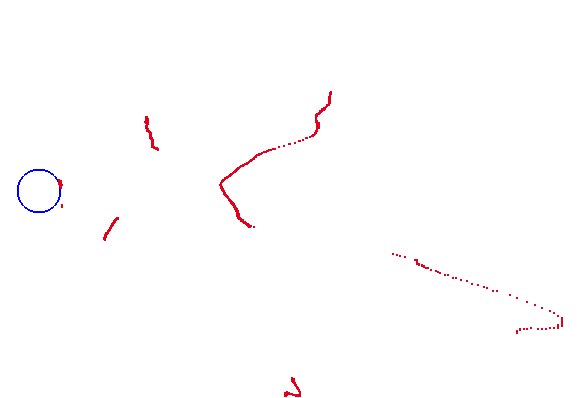
\includegraphics[width=\textwidth]{../Material/depth_slice.png}
    \caption{Top down view of the points used for the DBGridScan-Algorithm}
    \label{fig:det:dbtopdown}
\end{figure}

Most steps of the detection are done in two dimensions, assuming that the ground is at a constant height. 
Due to the introduction of slopes (see \ref{sec:det:ramp}) in 2017 this does not hold anymore. 
As a result the algorithm detects these slopes as obstacles. 
Furthermore it does not detect obstacles if these obstacles are at a different height than expected due to a slope.

To avoid false positives the detection is done at three heights independent of each other. 
Then it is checked for every obstacle if it is present on all three heights, for slopes this is not the case. 
This solves the problems related to false positives but does not help with the true negatives: obstacles which do not get detected as they are at a different height than expected due to a slope.

\subsection{Sign Detection}
As the computer on the vehicle has only a limited amount of computational resources the detection can not be done with state of the art detectors such as R-CNN \cite{rcnn}, Single-Shot-Detector \cite{ssd} or YOLO \cite{yolo}. The detection of the traffic signs is done with the depth data of the \ac{d435}. The detection estimates a bounding box for the signs, this bounding box gets mapped into the image of the main camera and an image is extracted. This image is then classified using a \ac{cnn}.

Multiple lines are scanned in the depth image to find large differences in distance which resemble an edge.
With these edges bounding boxes for sign candidates are extracted, these candidates are filtered based on their size, position and form. The \ac{cnn} then determines if the candidate is a valid sign and the type of the sign if it is one.

\begin{figure}[h]
    \centering
    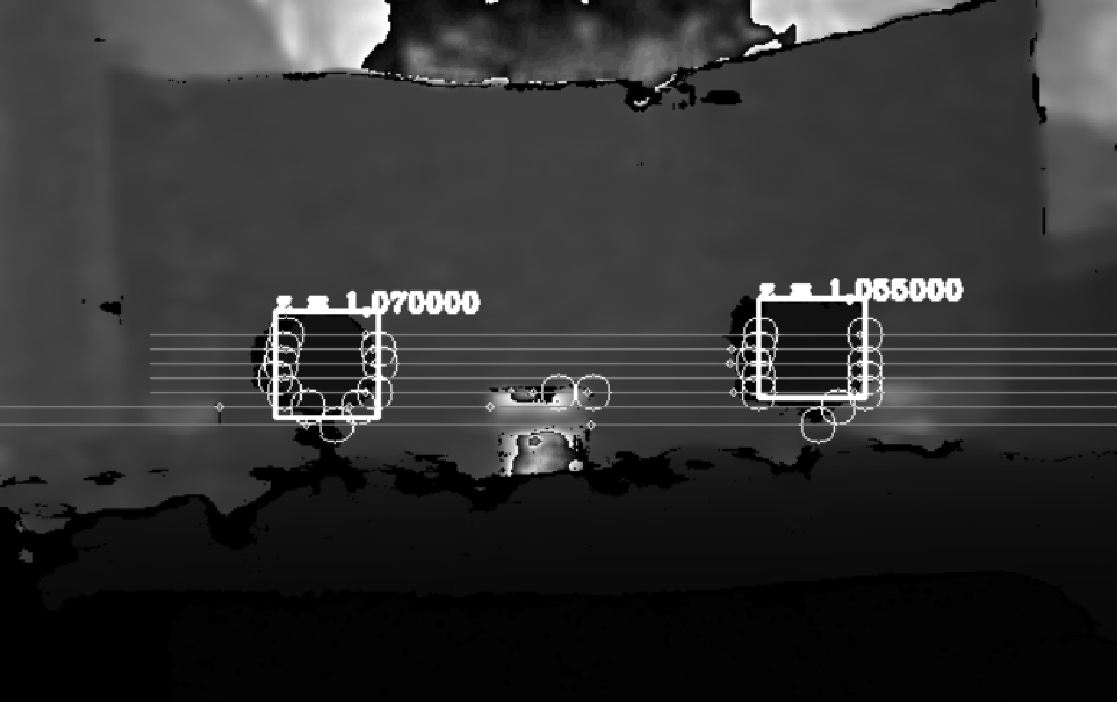
\includegraphics[width=\textwidth]{../Material/sign_depth_detection.png}
    \caption{Lines scanned by the sign detection}
    \label{fig:det:signScan}
\end{figure}

Figure \ref{fig:det:signScan} shows a disparity map of the camera. The lines along which the image is scanned, detected edges along these lines and filtered candidates are highlighted.

Similar to the obstacle detection the sign detection has difficulties with signs which are not on the expected height. Therefore some signs which are located on slopes do not get detected.

\subsection{Pedestrian Detection}
The detection of pedestrians is done twofold: as pedestrians are valid obstacles they get detected by the obstacle detection. 
This is done primarily to detect moving pedestrians at crosswalks. 
As there are no obstacles on crosswalks the contextual information can be used to differentiate between obstacles and pedestrians. 

Due to the small field of view of the \ac{d435}, pedestrians standing next to the road can not be detected by the obstacle detection. 
The detection of these pedestrians is done with a simple blob detector in the camera image if the vehicle is at a crosswalk.

\subsection{Slope Detection}
At the moment the slope of a ramp can not be detected by the vehicle. 
At the start of every slope there is a sign which signals the oncoming slope, if this sign is detected the vehicle decreases its speed.
Due to the problems listed above the sign is often not detected. Additionally there are problems with the lane and road markings detection on the ramp, this is because the complete image is warped on the ramp and as a result the extrinsic calibration is wrong and distances are estimated wrongly.

\section{Related Work}
In recent years many algorithms for object detection in point clouds have been proposed. 
Most of them do an end-to-end detection using a large \ac{cnn} \cite{Yin17} \cite{Bin19} \cite{Mar18} \cite{Li16}, for these networks the data is usually represented by voxels, which are pixels in the three dimensional space, or by a two dimensional map-like representation.
Due to the limitations in computational performance on the vehicle and the real time constraints it is not possible to use such a deep neural network for this task.
Faster algorithm rely on a separate detection and classification of the objects: first objects are detected in the point cloud, often using a clustering algorithm, then each cluster is classified.
For the clustering often an occupancy map is used, for most algorithms the classification is done with a learned classifier such as a support vector machine \cite{HivHWu10}, k-nearest neighbours \cite{YifeiTian18} or a \ac{cnn} \cite{AttBen17}.
Most of these algorithms are intended to be used with point clouds captured using a Lidar system.

For data acquired from stereo systems many algorithms use the disparity map for detection \cite{guindel18} \cite{qian16}. 
\cite{Wang19} discovered that the performance of object detection can be vastly improved by representing the data as a point cloud which correctly represents spatial relations, instead of disparity maps in which neighbouring pixels are not required to belong to the same object.

\section{Algorithm}
The following section introduces the proposed algorithm for object detection. 
The algorithm works in multiple steps: At first the algorithm decides for all points if it belongs to an object of interest, this step is referred to as segmentation. Next all points of interest are clustered to form objects. In the last step of the detection every cluster gets a type assigned. This is done by extracting a pseudo depth image for every cluster and classifying each depth image with a \ac{cnn}.

The algorithm is an improved version of \cite{AttBen17} to be used with point clouds generated from stereo systems instead of Lidar. 
It uses the point cloud as an input and detects the objects and determines the type of each object.
First the original algorithm is presented, then the improvements which enable the detection in stereo point clouds are presented.

Additionally to the improved algorithm of \cite{AttBen17} a bounding box is estimated for every cluster. Using points which do not belong to a cluster the ground is estimated by fitting a single plane.

\subsection{Segmentation}

\subsubsection{Grid}
All points of the point cloud are inserted into a grid. 
This is done by fitting a grid onto the $x$-$y$-plane, with the coordinate system defined like in section \ref{sec:theo:vehicleCoord}. 
The cells of the grid are equally sized. 
To reduce the number of points which need to be considered a region of interest for the grid is defined. 
For a point $\vec{p}$ given by $\vec{p} = {(x,y,z)}^\text{T}$, the region of interest is a function which defines for every
point if it is of interest:

\begin{equation}
    \text{ROI}\, (\vec{p}) = (0.2 \leq x \leq 3) \land (\abs{y} \leq 2) \land (-0.3 \leq z \leq 0.3)
\ \end{equation}

The cell a point belongs to is determined by projecting the point onto the $z=0$ plane. The point is then inserted into a set of points for the respective cell.

A cell $c$ is represented by a set of points:
\begin{equation}
    c = \{\vec{p}_1,\vec{p}_2, \ldots, \vec{p}_n \}\qquad \vec{p}_k \in \mathbb{R}^3,\ k \in \{1, \ldots, n\}
\end{equation}

\subsubsection{Classification}
The algorithm determines for every cell a type, the types are: Sparse, Low Foreground, High Foreground and Ground. 
The type Sparse is for cells which consist of few points, this is the case for cells which can not be seen by the sensor, either due to occlusion or due to the limited field of view.
The type Low Foreground is for all points which are part of an object such as cars and pedestrians, the type High Foreground is for points which belong to tall objects such as walls, the type Ground is for points which are part of the ground.

The type of each cell is calculated on the basis of the points in each cell. 
\cite{AttBen17} propose to determine the type of each cell based on the number of points, the minimum and the maximum height of all points in the cell. 

Cells with less than eight points are assigned the class Sparse. 
If the difference between the maximum and minimum height of the points in a cell is smaller than a predefined value the cell is labeled as ground.
A cell is classified as High Foreground if either the maximum height is larger than a threshold or the difference between the maximum and minimum height is larger than a threshold. 
All other cells are classified as Low Foreground.

\subsection{Clustering}
In the next step of the detection pipelines object candidates are extracted. This is done by clustering cells belonging to the class foreground. To improve the accuracy of the clustering it is done on a coarse and a fine level.

Two cells $c$ and $d$ belong to the same object if the coarse merging criterion $m_\text{Coarse}$ is fulfilled:
\begin{equation}
    m_\text{Coarse}\,  (c,d) = \abs{ \max_{{(x,y,z)}^\text{T} \in c}(z) - \max_{{(x,y,z)}^\text{T} \in d}(z) } < 0.05
\end{equation}
This yields clusters in which all cells have a similar maximum height. For the clustering the connected components labeling algorithm presented in section \ref{sec:theo:concomp} is used.

The coarse clustering limits the resolution of clusters to the size of a cell, to improve the accuracy clustering on a subcell level is performed. This is done by splitting every cell in a three times three grid, similar to the grid used for segmentation.

To be able to split objects which are close to each other \cite{AttBen14} proposed to do the second clustering step on the basis of the density of the cell. 
For this the ratio of the densities of two neighbouring cells is used. 
The criterion $m_\text{Fine}$, which indicates if two subcells $c$, $d$ belong to the same objects is:
\begin{equation}
    m_\text{Fine} = \frac{\max(\abs{c}, \abs{d})}{\min(\abs{c}, \abs{d})} < 10 
\end{equation}
This clustering step is only used to split objects which are close to each other, no existing clusters are merged.

\subsection{Extraction} \label{sec:det:originalExtraction}
After clustering each object needs to be classified. 
As small obstacles are of a similar size as signs it is not possible to classify the objects solely by size, the shape of the objects need to be taken into account as well. 
For such tasks \ac{cnn}s have proven to be a robust tool for classification.

As the algorithm is required to process frames in real time it is of great importance to reduce the time required by the \ac{cnn}.
The runtime of the classifier can be greatly reduced by reducing the number of inputs.
To achieve this the dimension of the input data has been reduced: instead of representing the data by the three dimensional point cloud of every cluster it is represented by a pseudo depth image of the cluster. \cite{AttBen17} try to ensure a side-view of the cluster by estimating the heading of the cluster.

To determine the heading the principal axes of the cluster are calculated. 
This is done by calculating the \ac{pca} over all points that are part of the cluster.
The \ac{pca} yields three eigenvectors $\vec{v}_1$, $\vec{v}_2$, $\vec{v}_3$ with three corresponding eigenvalues $\lambda_1$, $\lambda_2$, $\lambda_3$ and the mean of the cluster $\vec{p}_\text{mean}$.

The eigenvalues correspond to the variance of the cluster in the direction of the corresponding eigenvector. 
To represent this ordering the eigenvectors $\vec{v}_1$, $\vec{v}_2$, $\vec{v}_3$ are sorted in descending oder by the corresponding eigenvalues and then normalized, this yields the ordered and normalized eigenvectors $\vec{\tilde{v}}_1$, $\vec{\tilde{v}}_2$, $\vec{\tilde{v}}_3$.
To estimate the heading either $\tilde{v}_1$ or $\tilde{v}_2$ is chosen, this depends on their respective orientation. For this the angle $\alpha$ is calculated as the angle between the eigenvector and $z$-Axis:
\begin{equation}
    \alpha = \abs{
        \arccos \left(
        \begin{pmatrix} 
            0 & 0 & 1
        \end{pmatrix}
        \cdot \vec{\tilde{v}}_1
    \right)}
\end{equation}
For objects with the principal axis pointing primarily horizontally $\alpha$ is larger than $45^\circ$, in this case $\vec{v}_\text{side}$ is $\vec{\tilde{v}}_1$. For objects with the principal axis pointing primarily vertical ($\alpha < 45^\circ$), $\vec{\tilde{v}}_2$ is chosen as $\vec{v}_\text{side}$.

Using $\vec{v}_\text{side}$ the heading vector $\vec{v}_\text{heading}$ can be calculated as the horizontal vector pointing in the direction of the heading:
\begin{equation}
    \vec{v}_\text{heading} =
        \normalize{
            \begin{pmatrix}
                1 & 0 & 0 \\
                0 & 1 & 0 \\
                0 & 0 & 0
            \end{pmatrix}
            \cdot \vec{v}_\text{side}
        }
\end{equation}

For the calculation of the depth image all points need to be projected onto an image plane.
The axes of the depth image coordinate system are the heading of the cluster as the $x$ axis and ${(0,0,-1)}^\text{T}$ for the $y$ axis, the $z$ axis is defined by $x \times y$.

All points are mapped into the depth image coordinate system. In this coordinate system the bounding box of the cluster is determined by the respective minimum and maximum values:
\begin{eqnarray}
    x_\text{min} &=& \min_{{(x,y,z)}^\text{T} \in c}(x) \label{eqn:det:minx} \\ 
    x_\text{max} &=& \max_{{(x,y,z)}^\text{T} \in c}(x) \\
    y_\text{min} &=& \min_{{(x,y,z)}^\text{T} \in c}(y) \\
    y_\text{max} &=& \max_{{(x,y,z)}^\text{T} \in c}(y) \label{eqn:det:maxy} \\
    z_\text{min} &=& \min_{{(x,y,z)}^\text{T} \in c}(z) \label{eqn:det:minz} \\
    z_\text{max} &=& \max_{{(x,y,z)}^\text{T} \in c}(z) \label{eqn:det:maxz} \\
\end{eqnarray}

As it is necessary for the \ac{cnn} to have an input of constant size all images have a width and height of $S$ pixels each, \cite{AttBen17} propose $S=96$. To guarantee a constant size, a scaling factor $s$ is used for the points in the cluster:
\begin{equation}
    s = \frac{S}{\max(x_\text{max} - x_\text{min}, y_\text{max} - y_\text{min})}
\end{equation}

Additionally an offset for both the $x$ and the $y$ axis is defined, this offset is used to position the object in the centre of the image:
\begin{eqnarray}
    x_\text{Offset} &=& \frac{S - (x_\text{max} - x_\text{min}) \cdot s}{2} \\
    y_\text{Offset} &=& \frac{S - (y_\text{max} - y_\text{min}) \cdot s}{2}
\end{eqnarray}

Now a point $\vec{p}_\text{Cluster} = {(x,y,z)}^\text{T} \in c$ can be transformed to a point $\vec{p}_\text{Image} = {(x,y)}^\text{T}$ in the image coordinate system (\ref{sec:theo:imageCoord}):
\begin{equation} \label{eq:det:trans}
    p_\text{Image} = 
    \begin{pmatrix}
        s & 0 & 0\\
        0 & s & 0\\
    \end{pmatrix} 
    \cdot \left(\vec{p}_\text{Cluster} - 
    \begin{pmatrix} 
        x_\text{min} \\ y_\text{min} \\ z_\text{min} 
    \end{pmatrix} 
    \right) + 
    \begin{pmatrix} 
        x_\text{Offset} \\ y_\text{Offset} 
    \end{pmatrix}
\end{equation}

The brightness of a point $p_\text{Cluster} = {(x,y,z)}^\text{T}$ is determined by the distance from the image plane:
\begin{equation} \label{eq:det:bright}
    \text{Brightness} \left( \begin{pmatrix} x \\ y \\ z \end{pmatrix} \right)  = \frac{z - z_\text{min}}{z_\text{max} - z_\text{min}}
\end{equation}

To extract the pseudo depth image all points of the cluster are transformed into the depth image coordinate system, their brightness is determined according to equation \ref{eq:det:bright}. 
If there are multiple points which get mapped onto the same pixel the pixel closest to the vehicle, i.e. the pixel with the lowest brightness is used.

\subsection{Classification}
The classification is done with a \ac{cnn}. 
The network differentiates between the classes vehicle, pedestrian, short facade and street clutter. 
The \ac{cnn} consists of four convolutional layer, with max pooling after each layer, followed by a fully connected layer.

\section{Improvements}
Point clouds acquired by stereo systems pose different problems than those acquired with Lidar sensors. 
The number of outliers, that are points that do not belong to any object, is larger for stereo point clouds \cite{Wang19}. 
Furthermore these point clouds are dense, that means the density of points is high in comparison to the Sparse point clouds recorded with Lidar scanners.

\subsection{Segmentation}
Instead of using the four classes Sparse, Ground, Low Foreground and High Foreground it is sufficient to only consider three classes Sparse, Ground and Low Foreground for the Carolo Cup as there are no tall objects. In the following section the class Low Foreground is referred to as Foreground.

The minimum and maximum height of the points in a cell is determined by a single point in the cell. 
Due to the, in comparison to Lidar, large number of outliers in the point cloud it is not feasible to determine the type using the properties of a single point. 
By using the minimum and maximum heights of the points in each cell \cite{AttBen17} try to describe the properties of the distribution of the points along the $z$-Axis.
The distribution can also be described by statistical measures, such as the mean and the standard deviation, which are more robust to outliers. Thus the differentiation between ground and foreground cells is done by applying a threshold to the standard deviation of the height of all points in a cell.

As the number of points is a robust feature, that means it is not prone to a small number of outliers, the number of points can be used for the detection of sparse cells.

\subsection{Extraction}
All objects of the Carolo-Cup can be differentiated best from the front,
thus the image is extracted from a cluster $c$ by projecting all points of the cluster onto the frontal plane of the cluster, this simplifies the extraction.

For the input $S$ is chosen as 40, this size is sufficient to differentiate the objects by shape while keeping the input for the \ac{cnn} small, and thus reducing the runtime.

At a larger distance the density of the point cloud is lower than closer to the vehicle. 
This yields pixels in the image which do not show a point of the point cloud even though they show an object. 
To generate a distance invariant image a median filter of size 3x3 is applied to the image, this closes the holes in the image.
The density of the point cloud is sufficiently large that only single pixels are missing at the maximum distance, thus the kernel size of 3x3 is sufficient.

The median filter is a rank order filter, it takes all pixels in the neighbourhood of a pixel, orders them by brightness and sets the pixel to the median of this sorted list.

The point clouds calculated from the MEC-View system and the Kitti dataset contain additional colour information for each point. 
This colour information is used for the extraction of the patches, instead of a grey-scale image where each pixel represents a distance, the extracted patch is a colour image with the actual color of the points, thus the patches are depicting the object.

\subsection{Classification}
The Carolo-Cup Regulations (see section \ref{sec:det:ccr}) lists three objects which can occur on the track: Obstacles, Pedestrians and Signs. As Obstacles and Pedestrians are both represented by white boxes they can not be differentiated by size or shape, thus they are combined into one class. Additionally a class Clutter is added to represent objects which do not belong to any class. 

The size of the \ac{cnn} has been reduced to decrease the runtime.
The \ac{cnn} consists of two convolutional layers, with \ac{relu} as transfer function, each convolution uses 32 filters of size 3x3 each. For downsampling max pooling is used after each convolution. 
The convolutional layers are followed by two fully connected layers, the first consist of 128 neurons with the \ac{relu} transfer function. The classification is done by the last layer with three neurons. For these neurons softmax is used as a transfer function, so that the neurons represent a valid probability density function.
The structure of the \ac{cnn} can be seen in Figure \ref{fig:det:cnnStructure}.

\begin{figure}[h!]
    \centering
    \begin{tikzpicture}[scale=0.9]
        \node[anchor=south west,inner sep=0] at (0,0) {
            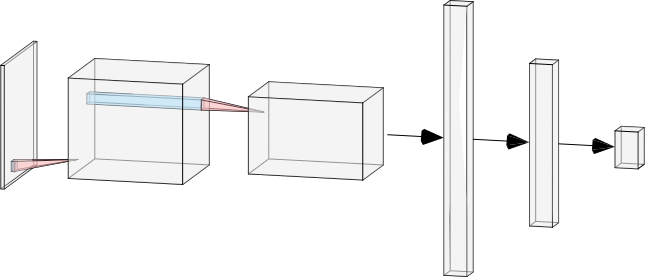
\includegraphics[width=.9\textwidth]{cnn.pdf}
        };

        \node at (1,-0.5) {Convolution};
        \node at (5,-0.5) {Convolution};
        \node at (9.5,-0.5) {Flatten};
        \node at (11.8,-0.5) {Dense};
        \node at (14,-0.5) {Dense};

        \node at (0.3,7) {$40\times40\times1$};
        \node at (3.3,7) {$20\times20\times32$};
        \node at (7.4,7) {$10\times10\times32$};
        \node at (10.8,7) {$3200$};
        \node at (12.8,7) {$128$};
        \node at (14.9,7) {$3$};
    \end{tikzpicture}
    \caption{Structure of the CNN (Graphic created using NN-SVG \cite{LeNail2019NN})}
    \label{fig:det:cnnStructure}
\end{figure}

The training data consists of $2,406$ hand labeled patches extracted from point clouds of the \ac{d435}. To enlarge the dataset the training data has been augmented by factor ten, this is done by mirroring the image along the $y$-axis, rotating the point cloud up to $10^\circ$ around the axes and adding noise to the image. From the training data 10\% of the data is used for verification during training to detect overfitting.

The \ac{cnn} has been trained over $200,000$ epochs using the Adadelta optimizer with cross entropy used as the loss. The learning rate started at 0.002, after $25,000$ epochs the learning rate was set to 0.0005 and after $55,000$ epochs it was reduced to 0.0001. During training both the accuracy, that is the number of correctly labeled images divided by the total number of images, and the loss for both the training and the validation data have been calculated to track the performance of the
\ac{cnn}.

\subsection{Bounding Box Estimate} \label{sec:det:bbe}
For the later stages of planning it is of great importance to not only know the position of objects but additionally the dimension and orientation of the objects. 
Especially for obstacles and pedestrians it is important to estimate the size, as these objects need to be passed.
For signs the bounding box is used as a region of interest for the following classification.
As both obstacles and pedestrians are box shaped the shape of objects is estimated by fitting a bounding box to the cluster.
The objects are always placed flat on the ground, thus the roll and pitch angles are assumed to be zero. 

The bounding box estimation is done in three steps: first the heading (yaw) of the bounding box is estimated, in the second step the size of the bounding box in the $x$ and $y$ dimension is estimated and in the last step the size in the $z$ dimension is estimated.

The heading vector is calculated using the \ac{pca}, identical to \ref{sec:det:originalExtraction}.
Using the heading vector the horizontal vector that is orthogonal to the heading vector can be calculated:
\begin{equation}
    \vec{v}_\text{orth} =
        \normalize{
            \begin{pmatrix}
                0 \\ 0 \\ 1
            \end{pmatrix}
            \times \vec{v}_\text{heading}
        }
\end{equation}

A point can now be transformed into the rotated coordinate system:
\begin{equation}
    \vec{p}_\text{transformed} =
        \begin{pmatrix}
            & \vec{v}_\text{heading} & \\ & \vec{v}_\text{orth} & \\ 0 & 0 & 1
        \end{pmatrix}
        \cdot \left( \vec{p} - \vec{p}_\text{mean} \right)
\end{equation}

By transforming all points of a cluster $c$ a transformed cluster $\tilde{c}$ can be calculated.
Using the transformed points the respective minimum and maximum values can be calculated similar to equation \ref{eqn:det:minx} to \ref{eqn:det:maxy}.
The maximum values can now be used to form the four corner points:
\begin{eqnarray}
    \vec{p}_{0,\text{transformed}} &=& 
        \begin{pmatrix}
            x_\text{min,transformed} \\ y_\text{min,transformed} \\ 0
        \end{pmatrix} \\
    \vec{p}_{1,\text{transformed}} &=& 
        \begin{pmatrix}
            x_\text{min,transformed} \\ y_\text{max,transformed} \\ 0
        \end{pmatrix} \\
    \vec{p}_{2,\text{transformed}} &=& 
        \begin{pmatrix}
            x_\text{max,transformed} \\ y_\text{max,transformed} \\ 0
        \end{pmatrix} \\
    \vec{p}_{3,\text{transformed}} &=& 
        \begin{pmatrix}
            x_\text{max,transformed} \\ y_\text{min,transformed} \\ 0
        \end{pmatrix}
\end{eqnarray}
This guarantees, that all points are inside of the bounding box.

By transforming the corner points back into the original coordinate system the bounding box can be calculated:
\begin{equation}
    \vec{p} = {
        \begin{pmatrix}
            & \vec{v}_\text{heading} & \\ & \vec{v}_\text{orth} & \\ 0 & 0 & 1
        \end{pmatrix}
    }^{-1} \cdot \vec{p}_\text{transformed} + \vec{p}_\text{mean}
\end{equation}

For the dimensions of the bounding box along the $z$-Axis the minimum and maximum values are calculated identical to equation \ref{eqn:det:minz} and \ref{eqn:det:maxz}. These two values are selected as the height of the bottom and top of the bounding box.

\subsection{Ground Estimate}
For the detection of the slope the ground plane is approximated by a single plane. 
At the beginning of a slope the ground consists of two slopes, thus the single plane is not able to perfectly fit the ground. As the ground estimate is only used as a binary detector for the slope, the angle of the slope is not important, this accuracy is still sufficient.

To fit the plane all cells labeled as ground are taken into account. For each cell a single point is determined by the centre of the cell and the average $z$ values of all points in the cell. In contrast to using all points which are part of a ground cell this approach is not influenced by the varying density of the point cloud. Thus the plane is not biased towards the ground points closer to the vehicle.

The plane is chosen such that, the average squared error between the points and the plane is minimal. The algorithm used for this least squares approach is the algorithm presented in Section \ref{sec:theo:leastSquaresPlane}.

\chapter{Evaluation} \label{sec:eval}
In the following chapter the performance of the algorithm is evaluated. 
The first section is a quantitative evaluation of the different steps of the pipeline and the end-to-end detection performance. The second
section evaluates the performance and highlights the strengths and weaknesses of the detection. In the third section
the computational performance, that is primarily the required time for the different steps, gets evaluated. In the next section the performance on
real world data is evaluated. Two different datasets are chosen: first the data acquired by a stereo camera in Ulm-Lehr as part of the MEC-View-Project \cite{mec} and second data from the Kitti dataset \cite{Menze2015CVPR}.  
Lastly the runtime of the algorithm is compared with other state of the art algorithms.

\section{Quantitative Evaluation}
To evaluate the performance of the algorithm 20 point clouds recorded on the vehicle with the \ac{d435} have been labeled by hand, in total there are 47 objects of interest in these point clouds. The point clouds show 22 obstacles and pedestrians and 25 signs. Ten of the 20 point clouds are recorded on the slope or show parts of the slope.
In each point cloud every point has been assigned one of the following classes:
\begin{itemize}
    \item Ground
    \item Sign
    \item Obstacle/Pedestrian
    \item Street Furniture
    \item Clutter
\end{itemize}
Obstacles and pedestrian are combined in one class as it is not possible to discriminate between them solely from the point cloud. 
The class "Clutter" represents all points that are outliers and thus do not belong to any class, Figure \ref{fig:eval:typeSparse} shows an example for such outlier points.
In contrast the class "Street Furniture" represents all points which are valid but do not belong to objects which are of interest, these objects include
things such as guardrails and walls.

\subsection{Segmentation}
The segmentation is the first step of the detection pipeline. In this step every cell gets a type assigned. The type gets decided based on the variance of the height of the points in each cell.

The performance gets evaluated in two ways, first on a per point level, that means the class of every point is compared with the actual class.
The second way is the evaluation on a per cell level, that means every cell is compared with the class of the cell. The ground truth class of the cells is
determined by the class with the largest number of points in the cell. If a cell contains less than eight points it is classified as Sparse, this is identical to how it is done in the algorithm.

To be able to not only see the correct detection rate but also the failure modes the data is shown in a confusion matrix. The rows represent predictions, that is the output of the algorithm, the columns the actual type of the point or cell.
The matrix consists of the points of all 20 ground truth point clouds.

The types of the labeled points are not the same as the types of the points after segmentation. To compare the points, the types of the ground truth data get mapped on the segmentation types.
The mapping is as follows: Sign and Obstacle/Pedestrian get mapped to the type Foreground, Clutter gets mapped to Sparse. The type Street Furniture is ignored, as the type corresponds to 
different types which are not of interest.

\begin{table}[h!]
    \centering
    \begin{tabular}{c|rrrrrr}
        \toprule
        \diagbox{Predicted}{Actual} & \multicolumn{2}{c}{Ground} & \multicolumn{2}{c}{Foreground} & \multicolumn{2}{c}{Sparse} \\
        \midrule
        Ground & 958,704 & (92.1\%) & 3,436 & (2.0\%) & 12,224 & (53.3\%) \\ 
        Foreground & 70,293 & (6.8\%) & 164,209 & (97.9\%) & 10,416 & (45.4\%)  \\ 
        Sparse & 11,688 & (1.1\%) & 71 & (0.04\%) & 273 & (1.2\%) \\ 
        \midrule
        Total & 1,040,685 && 167,716 && 22,913 \\
        \bottomrule
    \end{tabular}
    \caption{Confusion matrix on per point level}
    \label{tab:eval:confPoint}
\end{table}

The confusion matrix on point level (Table \ref{tab:eval:confPoint}) shows
that for the classes Ground and Foreground most points get
classified correctly.
The precision for ground points is 92\%, for the points labeled as Foreground the precision is 98\%. 
For the points classified as Sparse only a small number of the points is actually labeled as Sparse.
This is due to the fact, that many points which are labeled as Sparse
are actually in a cell with relevant points and thus are classified as
this class. An example for this problem can be seen in Figure \ref{fig:eval:typeSparse}

\begin{figure}[h!]
    \centering
    \begin{tikzpicture}
        \node[anchor=south west,inner sep=0] at (0,0) {
            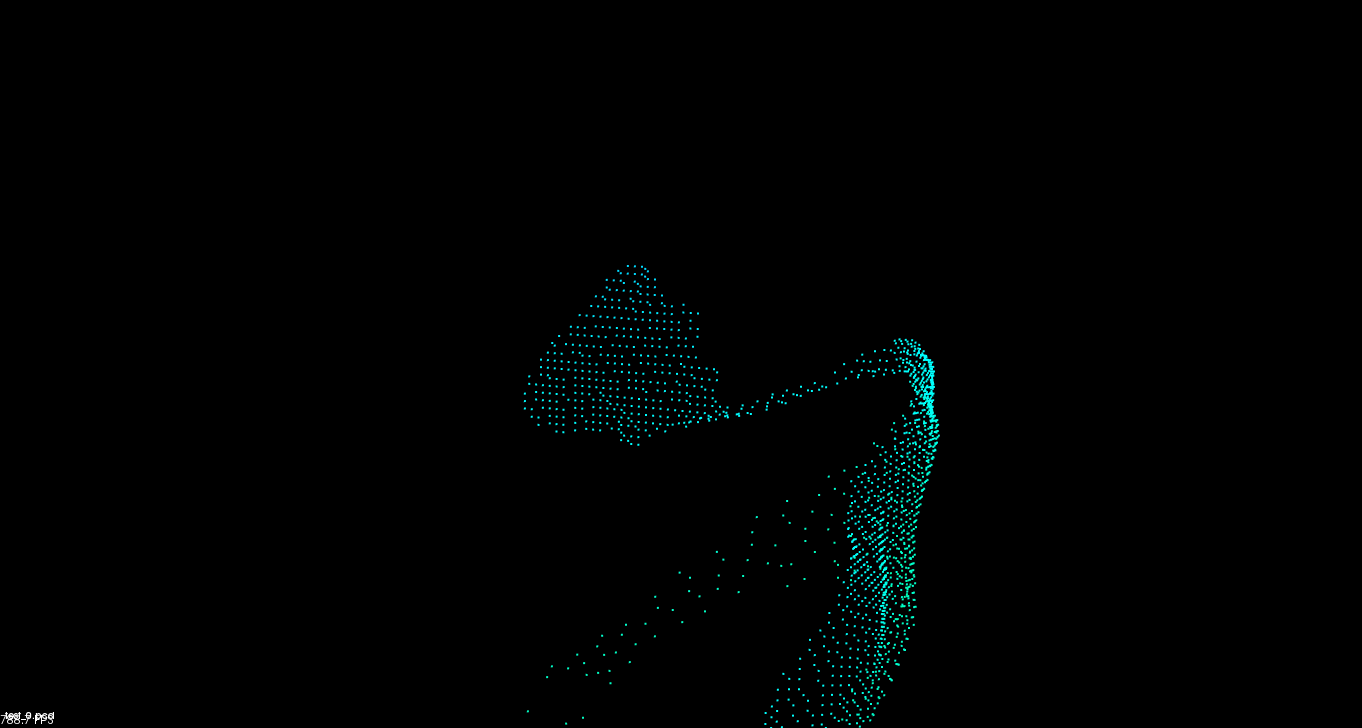
\includegraphics[width=\textwidth]{typeSparse.png}
        };
        \draw[draw=green, line width=0.1cm] (5.6,3.3) -- (8.3,3.3) -- (7.1,5.4) -- (5.6,3.3);
        \node at (5.5,4.5) {Sign};
        \draw[draw=red, line width=0.1cm] (9.2,4) ellipse (1.2 and 0.7);
        \node at (9.2,5.2) {Outlier};
    \end{tikzpicture}
    \caption{Outlier points next to a sign}
    \label{fig:eval:typeSparse}
\end{figure}

\begin{table}[h!]
    \centering
    \begin{tabular}{c|rrrrrr}
        \toprule
        \diagbox{Predicted}{Actual} & \multicolumn{2}{c}{Ground} & \multicolumn{2}{c}{Foreground} & \multicolumn{2}{c}{Sparse} \\
        \midrule
        Ground & 8,302 & (96.9\%) & 45 & (14.8\%) & 227 & (0.45\%) \\
        Foreground & 184 & (2.1\%) & 248 & (81\%) & 45 & (0.1\%) \\
        Sparse & 79 & (0.92\%) & 12 & (4.0\%) & 49,943 & (99.5\%) \\
        \midrule
        Total & 8,565 && 305 && 50,215 \\
        \bottomrule
    \end{tabular}
    \caption{Confusion matrix on cell level}
    \label{tab:eval:confCell}
\end{table}

For the classification on a per cell basis, the confusion matrix is shown in Table \ref{tab:eval:confCell}. 
The large number sparse cells in comparison to the number of sparse points is due to cells which do not contain any points, thus they are sparse but no points labeled sparse exist.
For all classes the majority of cells get labeled correctly. 
The precision for the ground cells is 97\%, for the classes labeled as Foreground the precision is 81\%, for the sparse cells the precision is 99\%.
The comparably high number of ground cells which have been labeled as Foreground is due to the outlier points (see Figures \ref{fig:eval:typeSparse} and \ref{sec:eval:outlier}).

When comparing the confusion matrices it can be seen that the precision on cell level is on average higher than those on the per point level. This is due to the non-uniformity of the cells, i.e. there are points of different classes in a single cell.

It can be concluded that the proposed heuristic yields a good precision for all classes. 
Especially the high precision for foreground points ($98\%$) provide a good basis for the object detection and clustering.

\subsection{Clustering and Bounding Box Estimation} \label{sec:eval:iou}
To assess the performance the \ac{iou} is calculated. 
This statistic measures the similarity of two sets by dividing the size of the intersection of both sets through the size of the union of both sets. 
For the bounding boxes the \ac{iou} is determined by the respective volumes.

The ground truth data is generated from the hand-labeled point clouds. Only objects which either belong to the class Sign or the class Obstacle/Pedestrian are considered for the evaluation.
For every object the bounding box is calculated identically to the real detection: the orientation of the box is estimated using the \ac{pca} of all points. The dimensions and
position are chosen such that all points of the cluster are in the bounding box.

The algorithm clusters all objects which belong to the class Foreground, as a result there are more bounding boxes in the detection than there are in the ground truth data.
For the evaluation only the relevant objects, that are the objects with the largest \ac{iou} relative to the ground truth, are used.

\begin{figure}[h!]
    \centering
    \begin{subfigure}[c]{0.75\textwidth}
        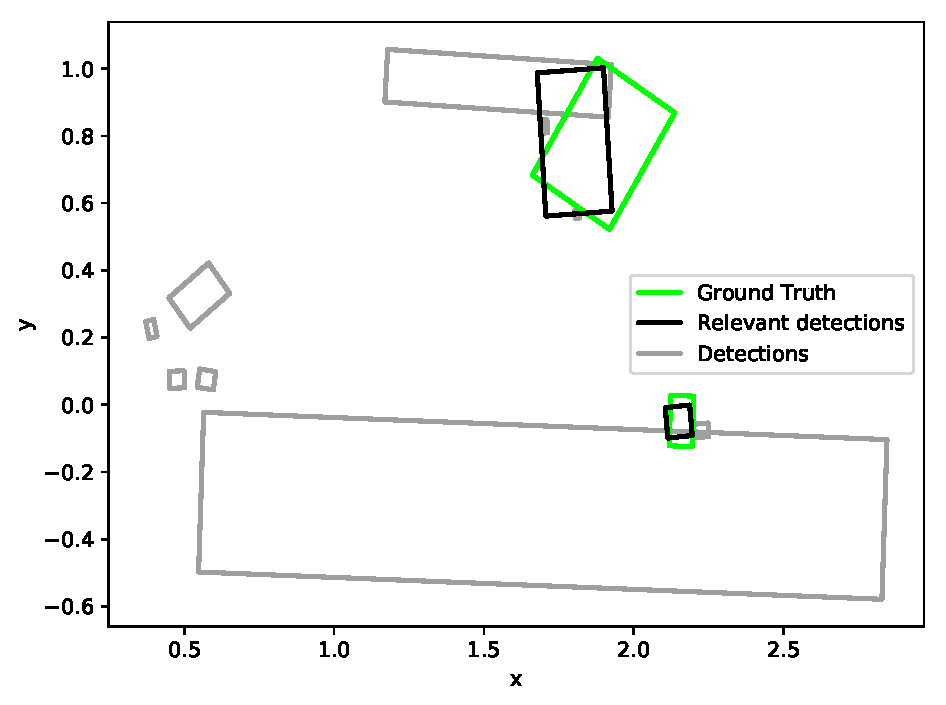
\includegraphics[width=\textwidth]{../Material/iou0.pdf}
        \subcaption{}
        \label{fig:eval:iou:0}
    \end{subfigure}

    \begin{subfigure}[c]{0.75\textwidth}
        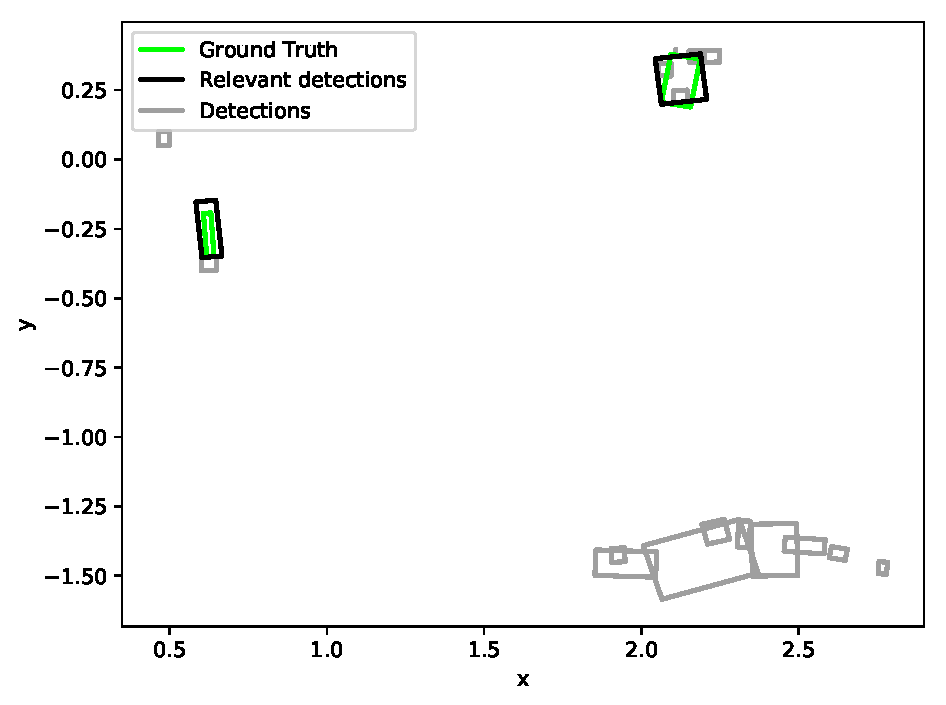
\includegraphics[width=\textwidth]{../Material/iou2.pdf}
        \subcaption{}
        \label{fig:eval:iou:2}
    \end{subfigure}
    \caption{Comparison of the estimated bounding boxes and the ground truth data, seen from above.}
    \label{fig:eval:iou}
\end{figure}

The \ac{iou} is calculated in 2D and 3D. For the 2D case the z-Axis is ignored and the \ac{iou} is only calculated by area as it can be seen in Figure \ref{fig:eval:iou}.
This information is the relevant information for the later stages of planning which are done solely in 2D. To evaluate the true performance the 3D bounding boxes are evaluated as well,
for this step the \ac{iou} is calculated based on the respective volumes.

Both \ac{iou}-scores are calculated for all 47 objects in the 20 ground truth point clouds. 
The average \ac{iou} for both cases can be seen in Table \ref{tab:eval:iou}.
The histogram of the respective values can be seen in Figure \ref{fig:eval:iouDist}.

\begin{table}[h!]
    \centering
    \begin{tabular}{cc}
        \toprule
        Average 2D & 0.444 \\
        Average 3D & 0.321 \\
        \bottomrule
    \end{tabular}
    \caption{Average IoU Scores} 
    \label{tab:eval:iou}
\end{table}

\begin{figure}[h!]
    \centering
    \begin{subfigure}[c]{0.49\textwidth}
        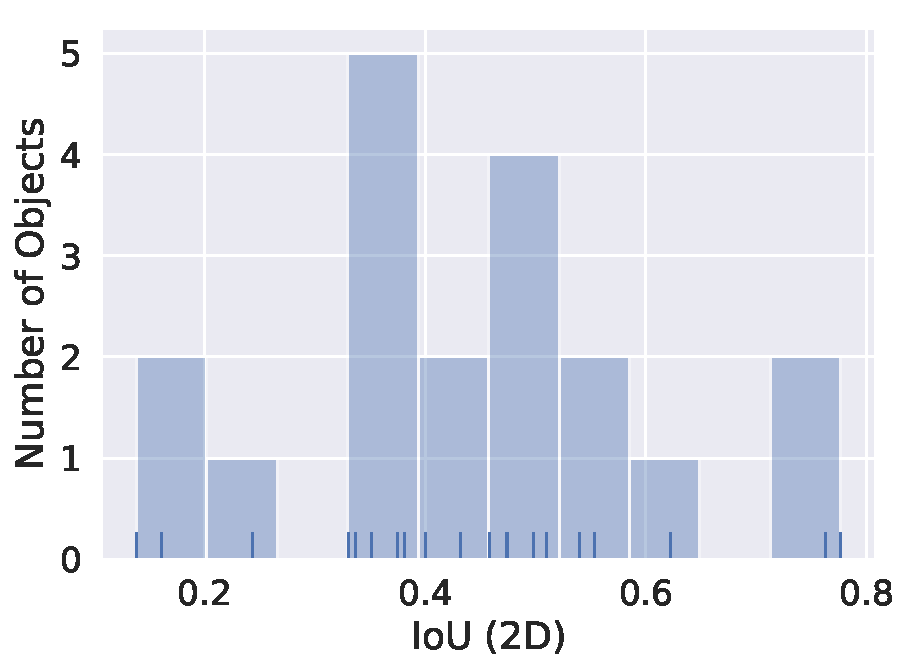
\includegraphics[width=\textwidth]{../Material/iouDist2.pdf}
        \subcaption{2D}
    \end{subfigure}
    \begin{subfigure}[c]{0.49\textwidth}
        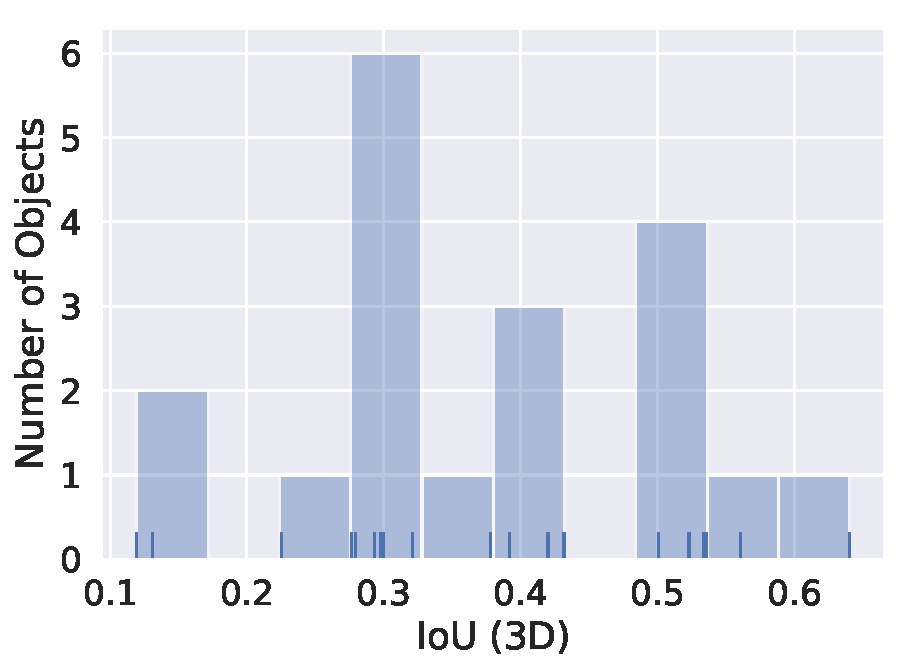
\includegraphics[width=\textwidth]{../Material/iouDist3.pdf}
        \subcaption{3D}
    \end{subfigure}
    \caption{Distribution of the IoU-Scores}
    \label{fig:eval:iouDist}
\end{figure}

The \ac{iou}-Scores are quite low when compared to typical values for computer-vision tasks, this is due to the two major differences: first the heading for the bounding box is not fixed, as a result the bounding boxes can be rotated relative to each other, this can be seen for the upper bounding box in Figure \ref{fig:eval:iou:0}, which only yields an 2D-\ac{iou} of 0.42.
The second difference is the third dimension, which leads to a smaller \ac{iou} as well.

It is clearly visible that the histogram for the three dimensional \ac{iou} is shifted to the left when compared with the one for the two dimensional case. This shows that the values for the 3D case are in general lower than the values for the 2D case.

Figure \ref{fig:eval:iou} shows that for most objects the bounding box is larger than ground truth bounding box. Thus obstacles can be passed reliably without touching them, as the minimum distance between obstacles is $1\si{\m}$ \cite{Carolo-CupRegelwerk} the large bounding box is not an issue. For signs a large bounding box results in a large region of interest, this simplifies the classification as the complete sign is inside the bounding box.

\subsection{Classification}
For every cluster an image is extracted and used for classification. The classification is done with a \ac{cnn}.

Every image is assigned one of three classes: Sign, Obstacle or Clutter. 
The class Obstacle includes pedestrians as well.

For evaluation a separate dataset which has not been used for training has been labeled.
It consists of 657 patches extracted from the 20 ground truth point clouds.
Of all patches 37 patches show objects of interest, that is obstacles and signs,
which have been detected by the algorithm. The number of patches is lower than the number of objects, this is because the algorithm is not able to detect every object correctly.

\begin{table}[h!]
    \centering
    \begin{tabular}{c|rrrrrr}
        \toprule
        \diagbox{Predicted}{Actual} & \multicolumn{2}{c}{Clutter} & \multicolumn{2}{c}{Obstacle} & \multicolumn{2}{c}{Sign} \\
        \midrule
        Clutter & 555 & (89.5\%) & 3 & (15.8\%) & 3 & (16.7\%) \\
        Obstacle & 49 & (7.9\%) & 15 & (78.9\%) & 1 & (5.6\%) \\
        Sign & 16 & (2.5\%) & 1 & (5.2\%) & 14 & (77.8\%) \\
        \midrule
        Total & 620 && 19 && 18 \\
        \bottomrule
    \end{tabular}
    \caption{Confusion matrix for the classification}
    \label{tab:eval:class}
\end{table}

Most of the relevant objects are classified correctly. The majority of patches that have been classified
wrong are Clutter which are either classified as Obstacles or Signs. 

By looking at the classification as a binary classification problem, that is by combining the classes Obstacle and Sign into one class "relevant" a second confusion matrix can be created, this can be seen in Table \ref{tab:eval:classBin}. 
Furthermore the precision, recall and $F_1$-score can be calculated \cite{informationRetrieval}. 
The recall is the number of correctly labeled patches divided by the total number of patches for this class. 
The $F_1$-score is the harmonic mean of precision and recall.
The results can be seen in Equation \ref{eqn:eval:classPrecision}.

\begin{table}[h!]
    \centering
    \begin{tabular}{c|rrrr}
        \toprule
        \diagbox{Predicted}{Actual} & \multicolumn{2}{c}{Relevant} & \multicolumn{2}{c}{Clutter} \\
        \midrule
        Relevant & 31 & (83.8\%) & 65 & (10.5\%) \\
        Clutter & 6 & (16.2\%) & 555 & (89.5\%) \\
        \midrule
        Total & 37 && 620 \\
        \bottomrule
    \end{tabular}
    \caption{Evaluation of the classification as binary classification problem}
    \label{tab:eval:classBin}
\end{table}

%https://medium.com/@jonathan_hui/map-mean-average-precision-for-object-detection-45c121a31173
\begin{eqnarray}
    \label{eqn:eval:classPrecision}
    \text{Precision} &=& \frac{31}{31 + 65} = 0.32\\
    \text{Recall} &=& \frac{31}{31+6} = 0.84 \\
    F_1 &=& 2 \cdot \frac{0.84 \cdot 0.32}{0.84+ 0.32} = 0.46
\end{eqnarray}

It is more important to detect all relevant objects than to achieve a high precision, thus the classification has been tuned to produce a high recall rate (84\%). The high number of false positives which result in a low precision can be tolerated because according to the Carolo-Cup rules \cite{Carolo-CupRegelwerk} there are no objects other than obstacles or signs on the road.

\subsection{Overall Performance}
The presented algorithm is an end-to-end approach for object detection in point clouds, thus the overall performance is evaluated.

The performance is evaluated similar to \cite{AttBen17}: for every object category the precision, recall and $F_1$-score is calculated. For the evaluation the detected object is compared with the object with the largest \ac{iou} in the ground truth data.

\begin{table}[h!]
    \centering
    \begin{tabular}{c|c|rrr}
        \toprule
        Category & Number of Objects & Pr & Rc & $F_1$\\
        \midrule
        Obstacle/Pedestrian & 20 & 100\% & 84\% & 91\% \\
        Sign & 18 & 78\% & 100\% & 88\% \\
        \midrule
        Average/Sum & 38 & 89\% & 92\% & 90\% \\
        \bottomrule
    \end{tabular}
    \caption{Overall performance of the proposed algorithm. Notations: Precision (Pr), Recall (Rc), $F_1$-score ($F_1$).}
    \label{tab:eval:overallProposed}
\end{table}

\begin{table}[h!]
    \centering
    \begin{tabular}{c|c|rrr}
        \toprule
        Category & Number of Objects & Pr & Rc & $F_1$\\
        \midrule
        Obstacle/Pedestrian & 20 & 100\% & 80\% & 89\% \\
        Sign & 17 & 71\% & 100\% & 83\% \\
        \midrule
        Average/Sum & 37 & 86\% & 90\% & 86\% \\
        \bottomrule
    \end{tabular}
    \caption{Overall performance of \cite{AttBen17}. Notations: Precision (Pr), Recall (Rc), $F_1$-score ($F_1$).}
    \label{tab:eval:overallBnb}
\end{table}

The performance of the proposed algorithm is shown in Table \ref{tab:eval:overallProposed} compared with the algorithm presented in \cite{AttBen17} which is shown in Table \ref{tab:eval:overallBnb}. 
Of the 47 objects in the 20 ground truth point clouds the proposed algorithm detects 38, the other algorithm detects only 37 objects. This yields an detection rate of 81\% and 79\% respectively.

For the average $F_1$-score the proposed algorithm is also superior to the detection presented in \cite{AttBen17}, with 90\% and 86\% respectively. On Lidar data \cite{AttBen17} achieves similar results, with a precision of 86\%, a recall of 83\% and a $F_1$-score of 85\%, albeit with four instead of three classes.

It should be taken into consideration that the dataset used for evaluation consists of less point clouds than the one used by \cite{AttBen17}.
Nonetheless the improvements of the algorithm result in a 2 percentage point higher detection rate, the precision is improved by 3 percentage points, the recall by 2 percentage points and the $F_1$-score by 4 percentage points.

\subsection{Ground Estimate}
For the evaluation all points of the 20 ground truth point clouds which are assigned the label ground are taken into account.
For each of these points the distance to the approximated plane is calculated.
Over all point clouds there are $1,691,693$ points which are part of the ground.

\begin{figure}[h!]
    \centering
    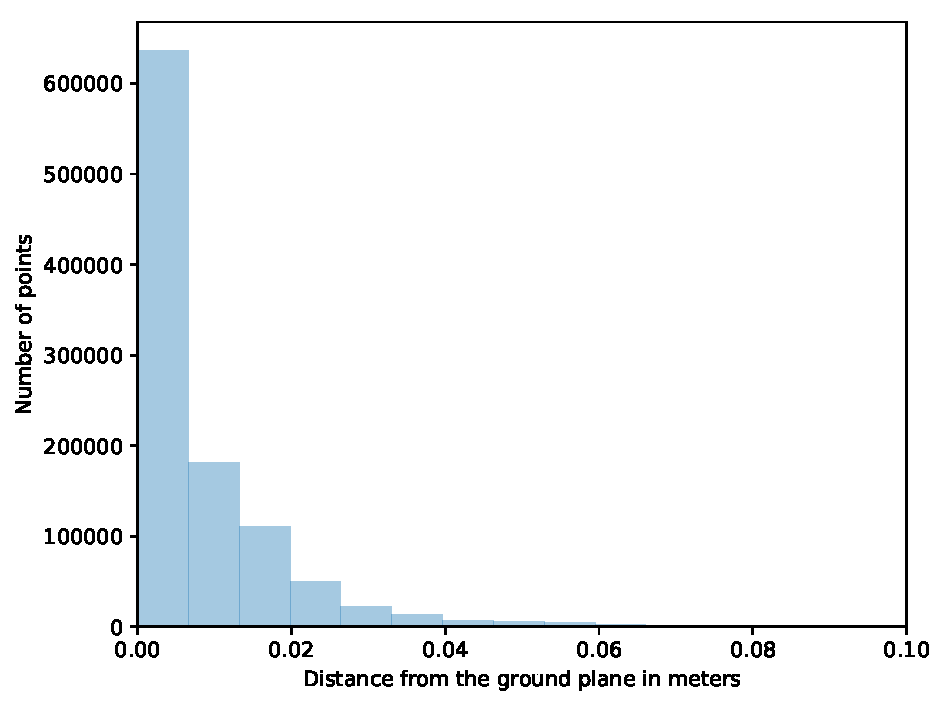
\includegraphics[width=\textwidth]{../Material/ground.pdf}
    \caption{Distribution of the distance to the plane}
    \label{fig:eval:groundDist}
\end{figure}

Figure \ref{fig:eval:groundDist} shows the distribution of the distances to the ground plane. 
It can be seen that most points are close to the estimated plane. Over all points the average absolute distance to the plane is 9.3 millimeters. The maximum error is 33cm, the point which yields this error is approximately $2\si{\m}$ from the vehicle after a slope on a flat part of the track, the estimated plane approximates the slope and not the flat part.

For situations in which the ground can not be approximated by a single plane the estimate yields the expected error. The plane has a slope, but the slope is smaller than the slope of the actual ground.
In situations in which the ground can be approximated by a single plane the error is small, in the ground truth data $71\%$ of all points are closer than $1\si{\cm}$ to the estimated plane. Thus the slope can be detected using the ground plane estimate. 

\subsection{Comparison with the current obstacle detection}
The proposed algorithm is intended to replace the obstacle detection currently used on the vehicle (see \ref{sec:det:obstDet}), thus the performance of the algorithms should be compared.
For the comparison the \ac{iou} scores are used, as described in section \ref{sec:eval:iou}.
The \ac{iou} is calculated in two ways: once only for the detected objects and second for all existing objects, objects that are not detected yield an \ac{iou} of $0$ for this score.

As the obstacle detection is intended to only detect obstacles, only clusters labeled as obstacles are taken into account. Over the 20 ground truth point clouds there are 22 objects labeled as obstacles. For the evaluation only the 2D-\ac{iou} is calculated as the current obstacle detection is not able to estimate the bounding box in three dimensions.

\begin{table}[h!]
    \centering
    \begin{tabular}{c|cc}
        \toprule
        Algorithm & \multicolumn{2}{c}{Average 2D-\ac{iou}} \\
         & Over detections & Over all objects \\
        \midrule
        Current obstacle detection & 0.48 & 0.087 \\
        Proposed & 0.44 & 0.38 \\
        \bottomrule
    \end{tabular}
    \caption{Comparison of the IoU-scores of the proposed algorithm versus the current obstacle detection}
    \label{tab:eval:compOld}
\end{table}

The current obstacle detection is only able to detect four of the 22 objects, the proposed algorithm detects 19 objects. The bad performance of the current obstacle detection is primarily due to the fact, that half of the ground truth point clouds are recorded on the slope which the current obstacle detection can not handle.

Table \ref{tab:eval:compOld} compares the \ac{iou} scores of both algorithm. 
For the \ac{iou} score calculated over the detections the current obstacle detection is marginally better than the proposed algorithm, but according to \cite{ioumurks}, even humans are not able to reliably differentiate an \ac{iou} of 0.3 from one of 0.5.
When considering all objects the proposed algorithm yields an higher \ac{iou} score than the current obstacle detection.

For the detected obstacles the difference in \ac{iou} scores is negligible.
When considering all objects, this is the case especially for situations involving the slope, the proposed obstacle detection yields a far better performance than the current obstacle detection. 

\section{Qualitative Evaluation}
In the following section the performance is evaluated qualitatively. For this certain difficult situations in which the algorithm performs well and situations in which the algorithm fails are shown and discussed.

\subsection{Failures}
\subsubsection{Clustering at Large Distance}
Large objects, such as walls, which are further away are often clustered into multiple objects. The wall in Figure \ref{fig:eval:pc1OverClustering} is
about three meters from the sensor. At this distance the distance to the
completely flat wall has a deviation of up to 0.3m. This leads to cells with a large variance in density which get clustered into different clusters.
Furthermore the sign in the foreground which can be seen in the bottom right
in Figure \ref{fig:eval:pc1OverClustering} casts a "shadow" onto the wall,
i.e. a frustum in the point cloud in which there are no points. This results in
a large change in density of the wall segment, which leads to multiple clusters.

As this only occurs for large objects which are far away, this doesn't influence the performance of the detection of relevant objects.
\begin{figure}[h!]
    \centering
    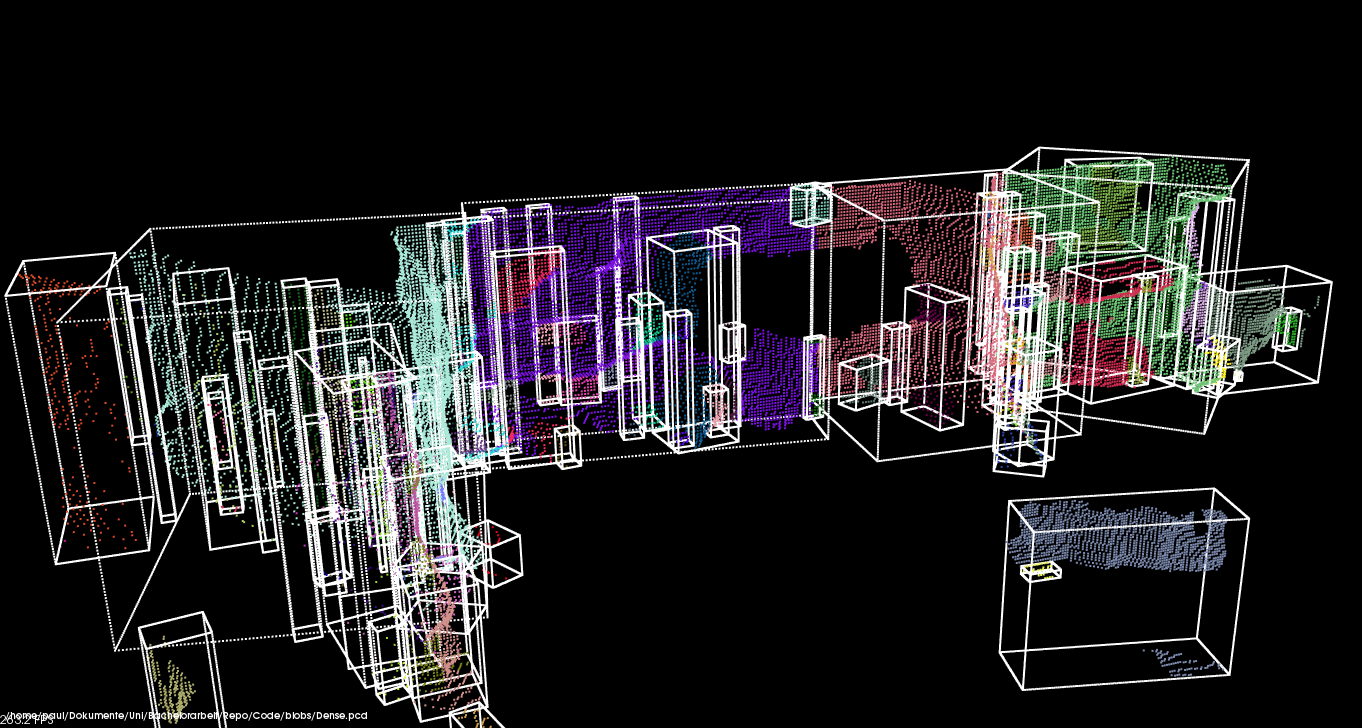
\includegraphics[width=\textwidth]{pc1OverClustering.png}
    \caption{The wall in the background is combined into many clusters}
    \label{fig:eval:pc1OverClustering}
\end{figure}

\subsubsection{Outliers} \label{sec:eval:outlier}
In the four corners of the depth-image there are a points with wrong depth estimates.
This leads to four rays consisting of these outliers in the point cloud. 
To remove these rays the point cloud gets cropped before inserting the points into the grid. 
The region of interest for cropping needs to be large enough to contain all points, even in extreme situations such as on the slope.
As a result some of these outlier points, especially close to the vehicle where they are close to the real points, are included in the region of interest.

This leads to the problem seen in Figure \ref{fig:eval:pc0Clutter}, the four small clusters in the foreground consist primarily of ground points.
But due to some outlier points below the relevant points the cells get classified as Foreground.

Due to the frequent occurrence of this problem there is sufficient training data for the \ac{cnn} which show such patches. As a result the cells with outliers get classified reliably as Clutter.
\begin{figure}[h!]
    \centering
    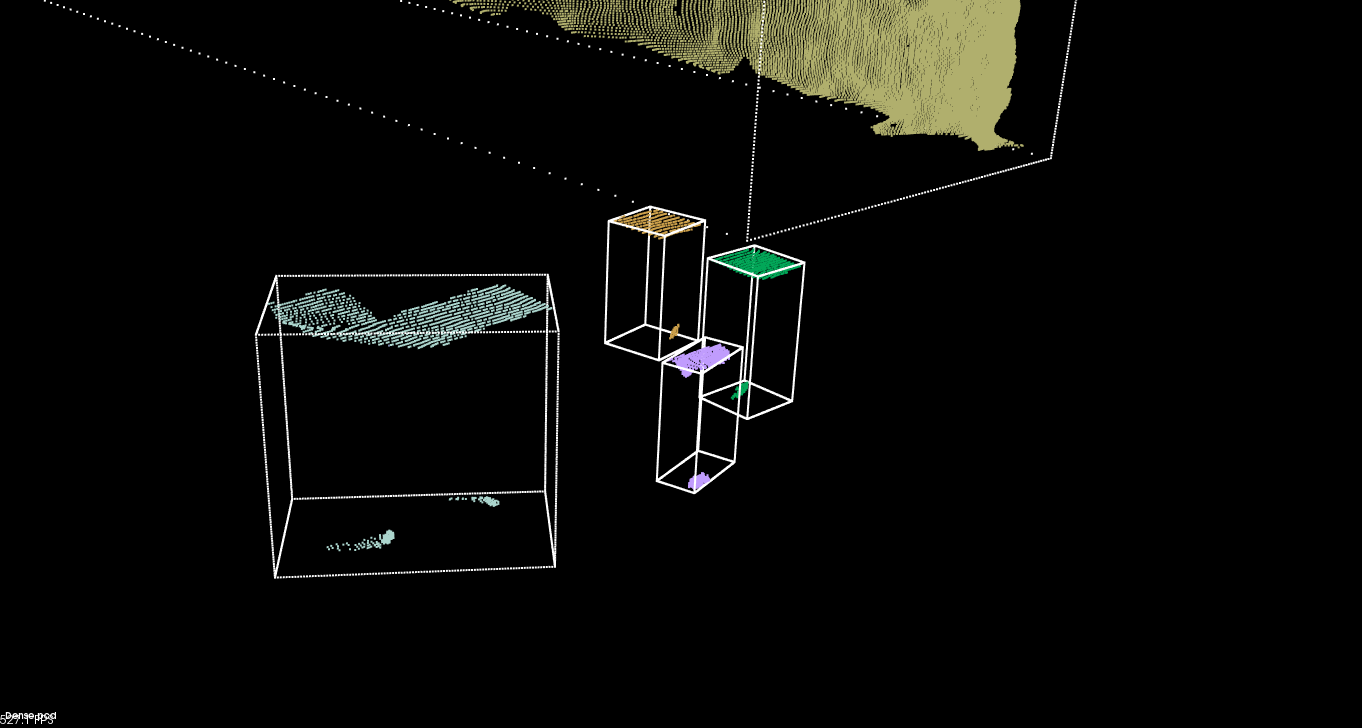
\includegraphics[width=\textwidth]{pc0Clutter.png}
    \caption{Clutter close to the vehicle}
    \label{fig:eval:pc0Clutter}
\end{figure}

\subsection{Expected Behaviour}
\subsubsection{Signs}
For obstacles and signs, such as the one shown in Figure \ref{fig:eval:pc1Sign} the bounding box is estimated correctly. 
As the bounding box is selected in such way that all points of the cluster lie within the box,
the later steps in the vehicle software, such as planning, have a good bounding box to avoid the obstacle.
Furthermore this provides a good region of interest for the classification of signs as the complete sign is visible in the extracted patch.

\begin{figure}[h!]
    \centering
    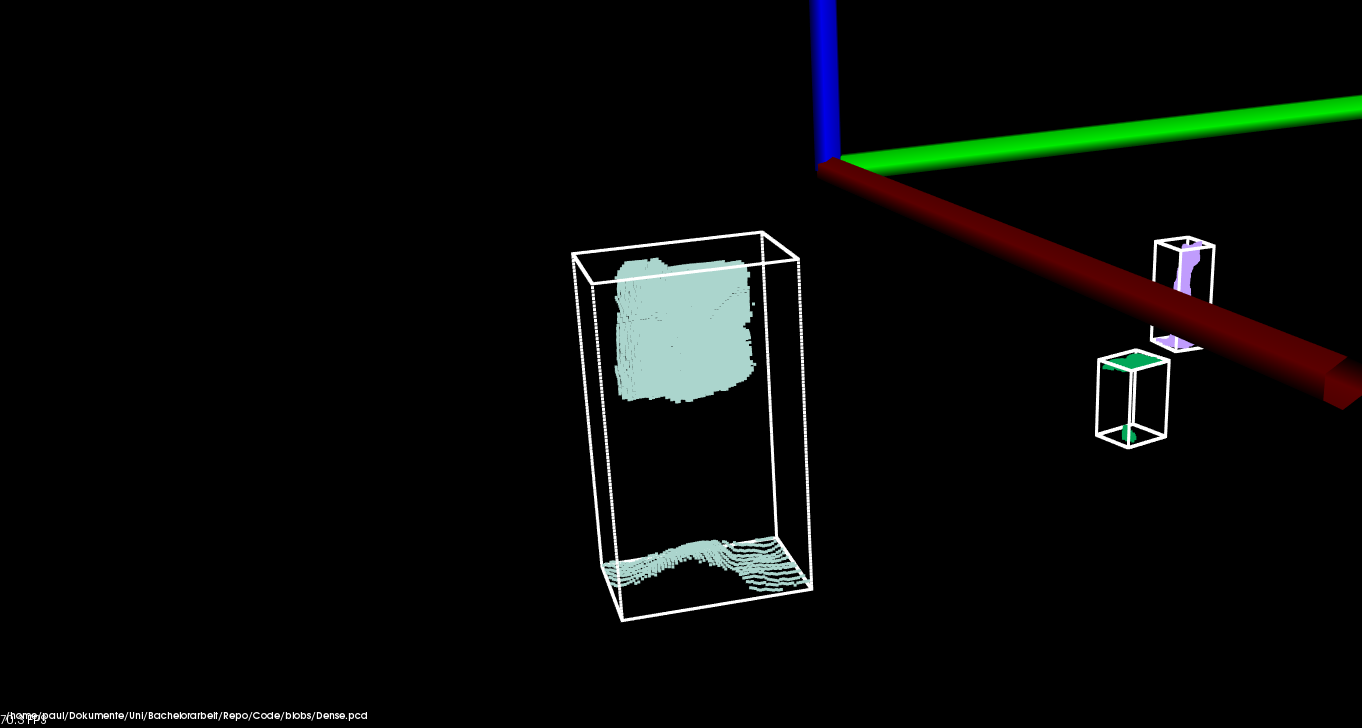
\includegraphics[width=\textwidth]{pc1Sign.png}
    \caption{Detected sign}
    \label{fig:eval:pc1Sign}
\end{figure}

\subsubsection{Obstacle touching the guardrail}
Figure \ref{fig:eval:pc0NotMerged} shows an obstacle touching the guardrail of the ramp, the guardrail is visible on the bottom left, the obstacle is in the centre of the image. 
In the point cloud there is no gap between the points which belong to the obstacle and the points which belong to the guardrail. 

In this difficult situation the separation of the two objects on subcell level is still possible due to the difference in density in both cells. As the obstacle is higher than the guardrail it contains more points and thus has a higher density. The current obstacle detection is not able to separate the objects.
\begin{figure}[h!]
    \centering
    \begin{tikzpicture}
        \node[anchor=south west,inner sep=0] at (0,0) {
            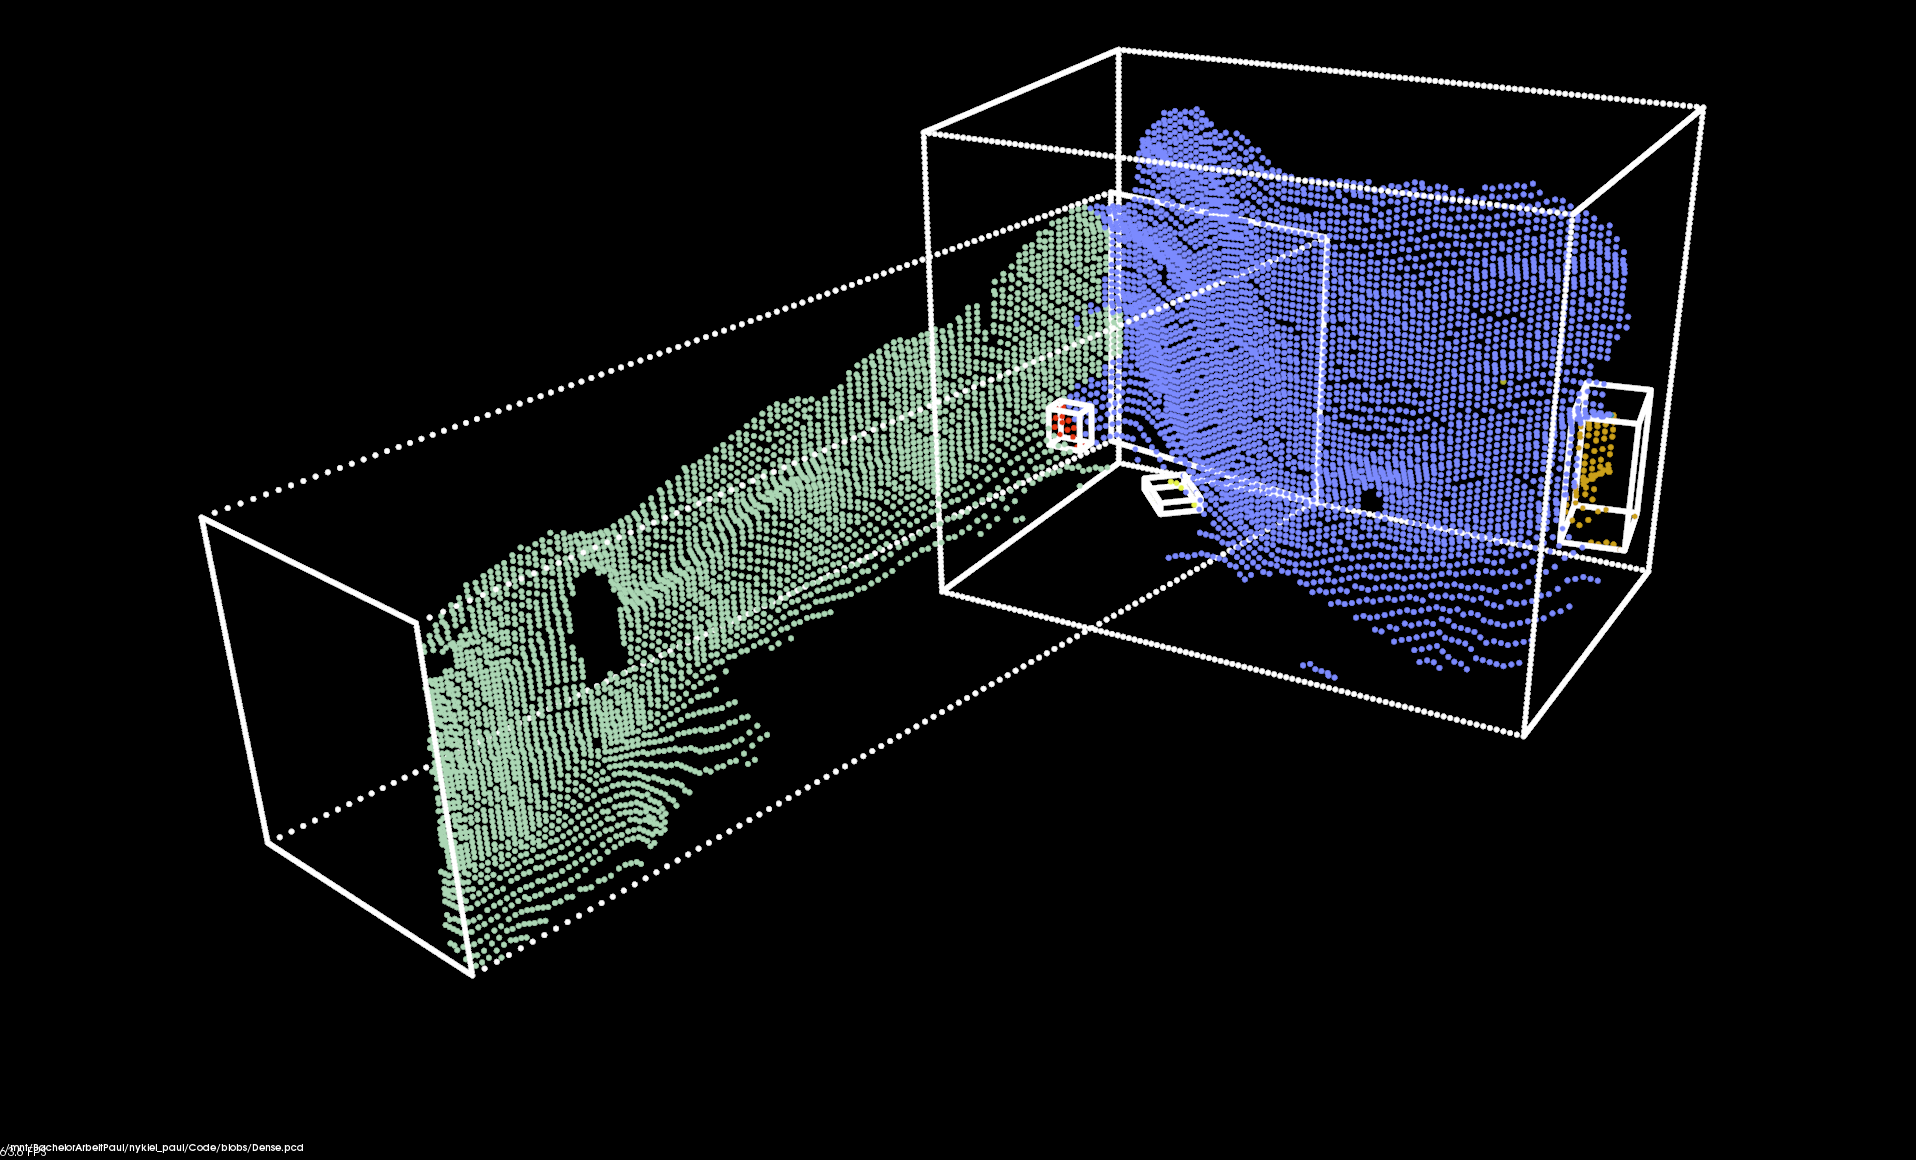
\includegraphics[width=\textwidth]{pc0NotMerged.png}
        };
        \node at (4,7) {Guardrail};
        \node at (11,9) {Obstacle};
    \end{tikzpicture}
    \caption{Obstacle close to the guardrail}
    \label{fig:eval:pc0NotMerged}
\end{figure}

\section{Computational Performance}
The \ac{d435} produces up to 30 frames per second at the maximum resolution, this limits the time for each run of the algorithm on a point cloud to 33ms.
Therefore it is required that the algorithm runs on average faster than 33ms.
In the following section the performance of the algorithm is evaluated.

\subsection{Setup}
The evaluation of the computational performance is done with a reference system similar to the system in the vehicle, as the vehicle was not available at the time of writing.
The system is equipped with an Intel\copyright Core\texttrademark i7-6700 CPU which similar in performance to the Intel\copyright Core\texttrademark i7-6770HQ CPU used in the vehicle.
The \ac{nuc} which is used in the vehicle only provides the integrated \ac{gpu}, there is no dedicated \ac{gpu}. 
Most frameworks used for neural networks, such as TensorFlow which is used here, require a Nvidia-\ac{gpu} which is able to use \ac{cuda} \cite{tensorflow2019}. As the integrated \ac{gpu} does not support \ac{cuda} it is not possible to accelerate the computations of neural networks. Therefore the \ac{gpu} in the reference system is not used for the evaluation.

Ubuntu 18.04 is used as the \ac{os}, with GCC-8 as the compiler for the software.

All steps of the algorithm are run sequentially to reduce the effects introduced by the scheduler of the \ac{os}.

\subsection{Overall Performance}
The runtime of the algorithm is measured on the 20 ground truth point clouds. 
To achieve more precise results the algorithm is run 100 times for every point cloud. 
Over all runs the mean and the standard deviation is calculated. 
Not only the overall runtime is measured but additionally the runtime for every part of the algorithm is measured.

\begin{table}[h!]
    \centering
    \begin{tabular}{l|S[table-format=2.2]S[table-format=1.3]}
        \toprule
         & {Average runtime} & {Standard deviation} \\
        \midrule
        Segmentation & 2.1ms & 0.49ms \\
        Clustering & 1.2ms & 0.52ms \\
        Extraction & 0.62ms & 0.25ms \\
        Classification & 15ms & 10ms \\
        Bounding Box Estimate & 0.73ms & 0.29ms \\
        Ground Estimate & 0.12ms & 0.046ms \\
        \midrule
        All & 19ms & 11ms \\
        \bottomrule
    \end{tabular}
    \caption{Runtime of the algorithm}
    \label{tab:eval:runtime}
\end{table}

The results can be seen in Table \ref{tab:eval:runtime}. 
Most of the time is used for the classification with the \ac{cnn}. 
The only other steps which require more than one millisecond on average is the creation of the grid and the clustering on the grid using connected components labeling on two levels. 
For the creation of the grid the most time is used for inserting all points in the grid, this is due to the large number of points. 
For the clustering the most time is used for the clustering of the fine clusters.

The average runtime is well below the time for one frame (33.3ms), this shows that the algorithm can be used on the vehicle.

\subsection{Runtime of the CNN}
As the \ac{cnn} is the part of the algorithm which requires by far the most time, its performance is evaluated in more detail.

Figure \ref{fig:eval:runtime_cnn} shows the runtime of the CNN for all patches against the number of patches. As expected the measurements are all more or less on a straight line, this shows that the runtime is proportional to the number of patches. 

\begin{figure}[h!]
    \centering
    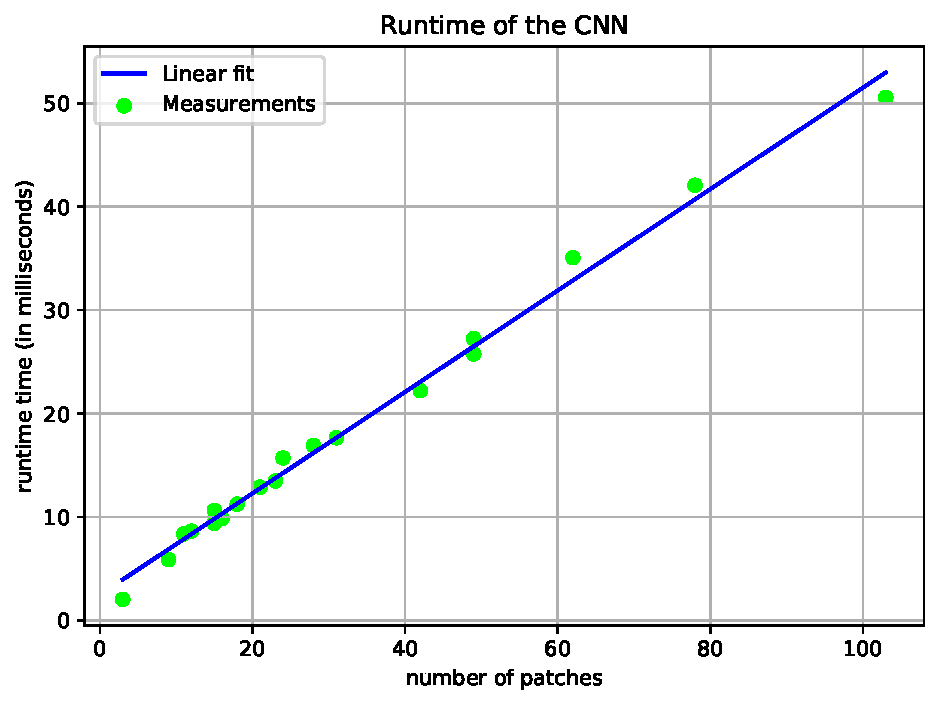
\includegraphics[width=\textwidth]{../Material/runtime_cnn.pdf}
    \caption{Plot of the runtime of the CNN against the number of patches}
    \label{fig:eval:runtime_cnn}
\end{figure}

Using least-squares regression a straight line can be fitted to the data. This line is given by:
\begin{equation}
    y = 0.49 \cdot x + 2.5
\end{equation}

The slope of the straight is 0.49 which is the average time in milliseconds per patch.

The average runtime of all steps of the algorithm but the CNN is on average 4.77ms. 
The maximum time the algorithm should require is 33ms, with these numbers the maximum number of patches which can be classified on average can be calculated:
\begin{equation}
    n_\text{max} = \frac{33 - 4.77}{0.49} = 57.6
\end{equation}

The clusters get extracted from the grid from near to far, the classification is started with objects which are closer to the vehicle. 
These objects are of greater importance, as these are the objects the vehicle has to handle first.

If the algorithm is required to finish in the given 33ms the classification can be stopped after a certain time. 
On average it is possible to classify 57 patches in this time frame. 
Compared to the relatively low number of relevant objects close to the vehicle this suffices to detect all relevant objects.

\section{Evaluation on real world data}
According to \cite{Wang19} object detection on stereo data can be vastly improved by representing the data as a point cloud instead of a disparity map. 
To verify this the algorithm should not only run on the data from the \ac{d435} but additionally on real world data.

The point clouds used as an input for the algorithm are calculated from two colour images. For the calculation of the disparity map semi-global block matching, an improved version of semi-global matching (see \ref{sec:theo:sgm}) is used.
From the disparity map the point cloud is calculated, as explained in \ref{sec:theor:disp2pc}.
In comparison to the data provided by the \ac{d435} no active stereo is used, the two cameras are the only source of depth information.

\subsection{Kitti}
The baseline of the camera system is only $0.54\si{\m}$ \cite{Menze2015CVPR}, as shown in \ref{sec:theo:error} the baseline distance is inverse proportional to the depth error.
As a result the quality of the point cloud is much lower than the quality of the point clouds acquired with the \ac{d435}. 
Figure \ref{fig:eval:kittiBadImage} shows a part of one of the two images used for the stereo extraction. 
The image is part of the Kitti dataset \cite{Menze2015CVPR}. 
Figure \ref{fig:eval:kittiBad} shows a part of the point cloud calculated from the stereo pair.

The scene shows two cars on the opposite side of the road. 
The car that is closer, marked in red, is about 13 meters from the camera. 
Even at this distance the point cloud does not show a single blob but multiple blobs around the actual position of the vehicle.

% Testing / 005 bzw. 2_11
\begin{figure}[h!]
    \centering
    \begin{tikzpicture}
        \node[anchor=south west,inner sep=0] at (0,0) {
            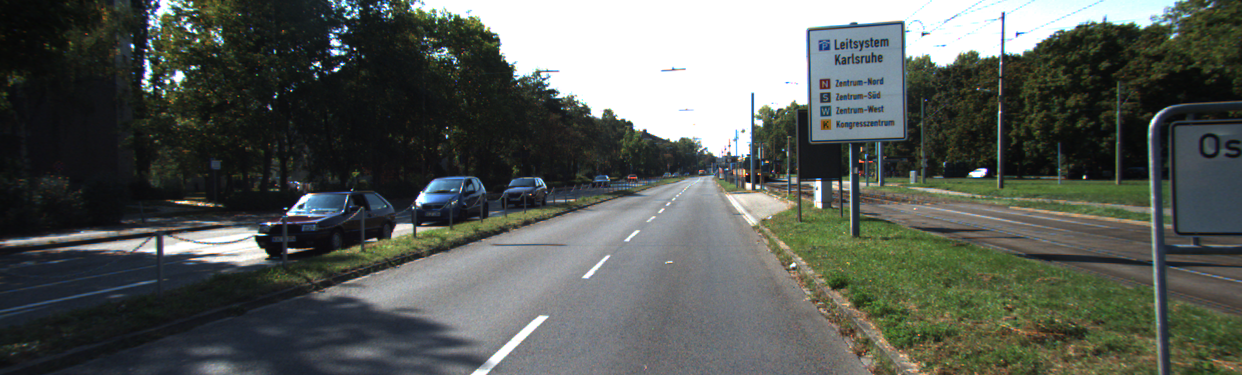
\includegraphics[width=\textwidth,trim={6cm 2cm 22cm 5cm},clip]{../Material/kittiBadImage.png}
        };
        \draw[red,ultra thick,rounded corners] (2.8,2) rectangle (7.7,4.5);
        \draw[green,ultra thick,rounded corners] (8.2,3) rectangle (10.8,5);
    \end{tikzpicture}
    \caption{Image from the Kitti dataset}
    \label{fig:eval:kittiBadImage}
\end{figure}

\begin{figure}[h!]
    \centering
    \begin{tikzpicture}
        \node[anchor=south west,inner sep=0] at (0,0) {
            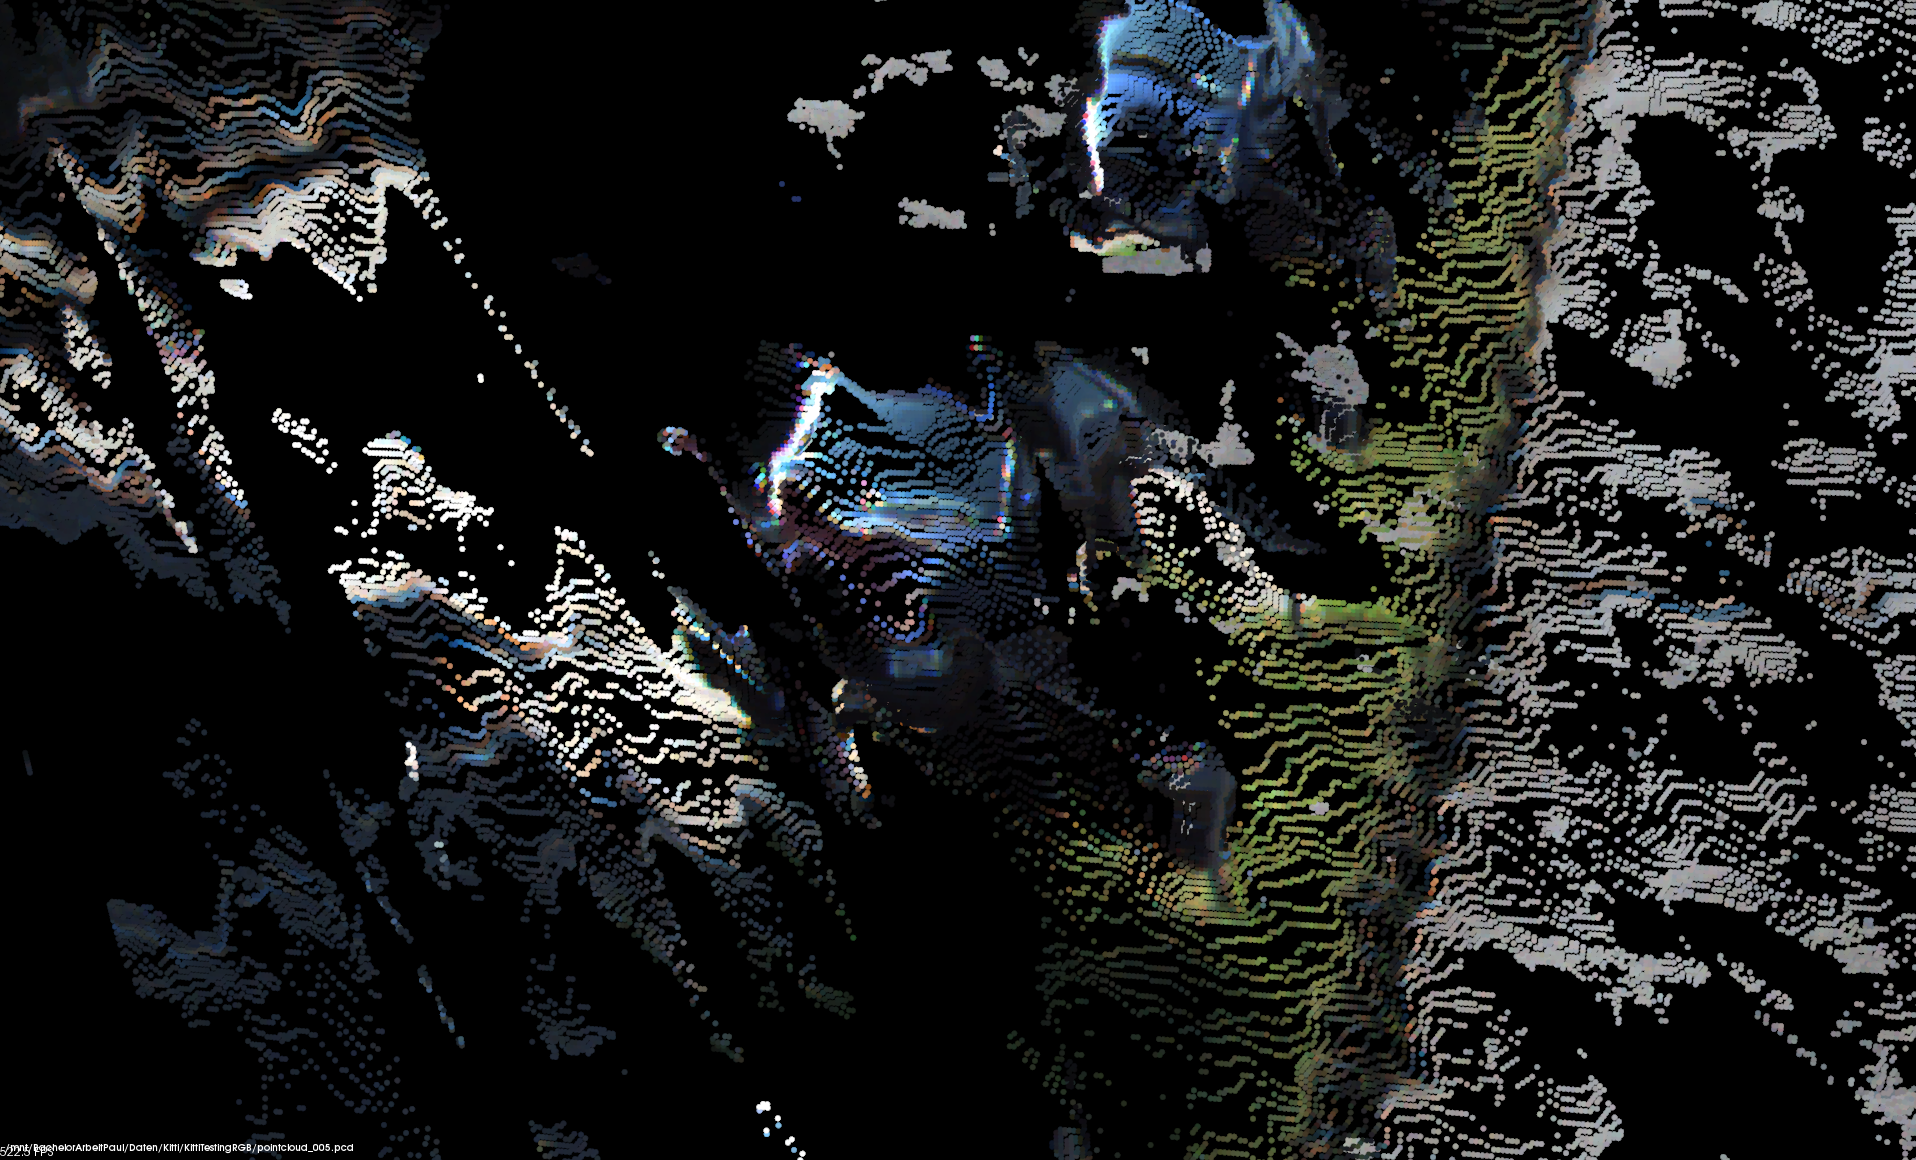
\includegraphics[width=\textwidth]{../Material/kittiBad.png}
        };
        \draw[red,ultra thick,rounded corners] (6,3.6) rectangle (9,6.6);
        \draw[green,ultra thick,rounded corners] (8.3,7.2) rectangle (10.5,9.2);
    \end{tikzpicture}
    \caption{Bird's-eye view of two vehicles in a point cloud generated from Kitti data}
    \label{fig:eval:kittiBad}
\end{figure}

The poor quality of the point cloud results in many small clusters due to the large variance in density throughout a single object. Therefore the patches that get extracted from the point cloud seldomly show the complete object, most of the time only parts of the objects are shown, subsequently the \ac{cnn} yields a poor performance.

To increase the accuracy of the classification the colour information of the point cloud is used to generate patches, which show the relevant object. Figure \ref{fig:eval:texture} shows examples for such patches.
The first row (Figures \ref{fig:eval:texture:222_0}, \ref{fig:eval:texture:222_0} and \ref{fig:eval:texture:0_0}) show all objects which are closer than 10 meters to the cameras.
The second row (Figures \ref{fig:eval:texture:0_1} and \ref{fig:eval:texture:0_1}) show objects at a larger distance.
For the objects closer than 10 meters the algorithm is able to correctly detect the objects and extract patches which show the complete vehicle. 
At a larger distance a single object in the point cloud is split up into multiple objects by the detection.
Therefore multiple patches which show only a part of the vehicle are extracted.

\begin{figure}[h!]
    \centering
    \begin{subfigure}[c]{0.3\textwidth}
        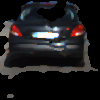
\includegraphics[width=\textwidth]{../Material/texture222_0.png}
        \subcaption{Car}
        \label{fig:eval:texture:222_0}
    \end{subfigure}
    \begin{subfigure}[c]{0.3\textwidth}
        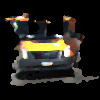
\includegraphics[width=\textwidth]{../Material/texture222_1.png}
        \subcaption{Van}
        \label{fig:eval:texture:222_1}
    \end{subfigure}
    \begin{subfigure}[c]{0.3\textwidth}
        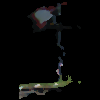
\includegraphics[width=\textwidth]{../Material/texture0_0.png}
        \subcaption{Sign}
        \label{fig:eval:texture:0_0}
    \end{subfigure}
    \begin{subfigure}[c]{0.3\textwidth}
        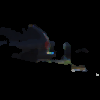
\includegraphics[width=\textwidth]{../Material/texture0_1.png}
        \subcaption{Rear of a car}
        \label{fig:eval:texture:0_1}
    \end{subfigure}
    \begin{subfigure}[c]{0.3\textwidth}
        
\includegraphics[width=\textwidth]{../Material/texture0_2.png}
        \subcaption{Centre of a car}
        \label{fig:eval:texture:0_2}
    \end{subfigure}
    \caption{Patches extracted from Kitti data}
    \label{fig:eval:texture}
\end{figure}

\subsection{Ulm-Lehr}
For the data acquired by the pilot installation in Ulm-Lehr the quality of the point cloud is better due to the larger distance of the cameras.
As the cameras are stationary they all show the same scene. The scene depicts a flat road with vehicles, no slopes are present. 
Due to the elevated mounting position of the camera system most parts of the road are visible at all times. 
In contrast objects in the Kitti dataset are often occluded by other objects.

The evaluation is done using the \ac{iou}, similar to section \ref{sec:eval:iou}. For the evaluation 2,322 labeled point clouds with 4,725 objects in total are used.
Out of the 4,725 objects 4,171 objects are detected by the algorithm, this is a detection rate of 88\%. 
Figure \ref{fig:eval:iouDistLehr} shows the histograms of the two- and three-dimensional \ac{iou}-scores, the average two dimensional \ac{iou}-score is 0.53, the average three-dimensional-score 0.43.

\begin{figure}[h!]
    \centering
    \begin{subfigure}[c]{0.48\textwidth}
        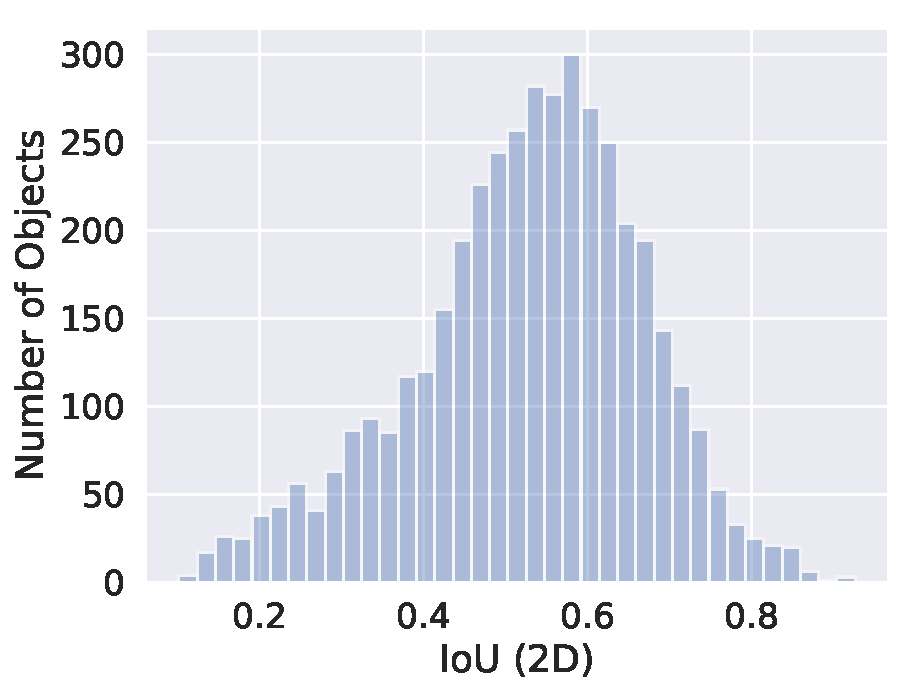
\includegraphics[width=\textwidth]{../Material/iou2_lehr.pdf}
        \subcaption{2D}
    \end{subfigure}
    \begin{subfigure}[c]{0.48\textwidth}
        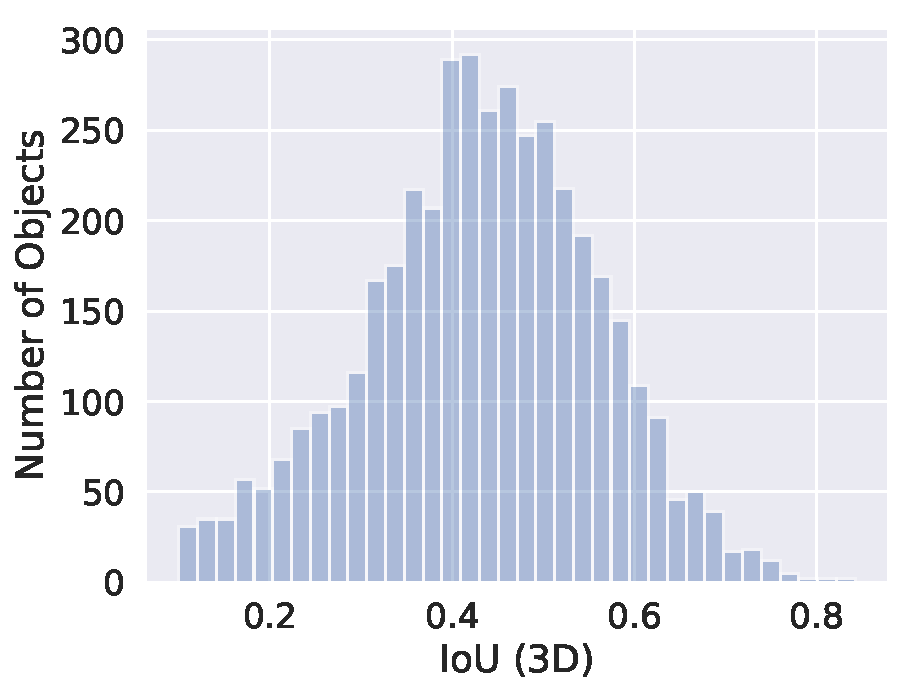
\includegraphics[width=\textwidth]{../Material/iou3_lehr.pdf}
        \subcaption{3D}
    \end{subfigure}
    \caption{Distribution of the IoU-Scores}
    \label{fig:eval:iouDistLehr}
\end{figure}

Both \ac{iou}-scores are higher than the respective score for the \ac{d435} data. This is primarily due to the simplicity of the scene and the elevated camera position.

Figure \ref{fig:eval:iouLehr} shows examples of the detections and the corresponding ground truth data. Objects closer than 50 meters, such as the ones shown in Figure \ref{fig:eval:iouLehr:2} generate an accurate bounding box. At distances over 50 meters, some objects can still be detected, like the object seen in \ref{fig:eval:iouLehr:1} but there is some noise present.

\begin{figure}[h!]
    \centering
    \begin{subfigure}[c]{0.75\textwidth}
        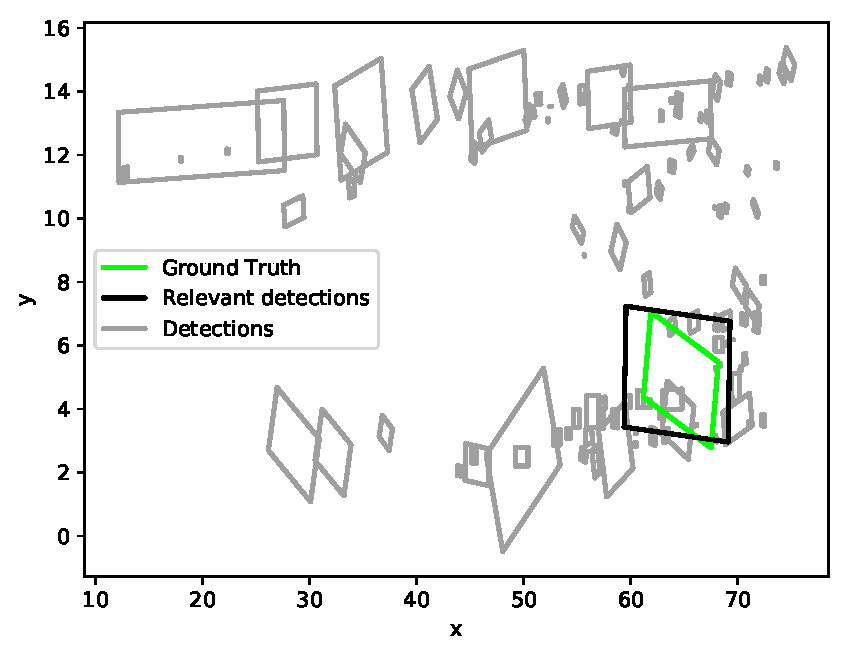
\includegraphics[width=\textwidth]{../Material/lehr1.pdf}
        \subcaption{}
        \label{fig:eval:iouLehr:1}
    \end{subfigure}
    \begin{subfigure}[c]{0.75\textwidth}
        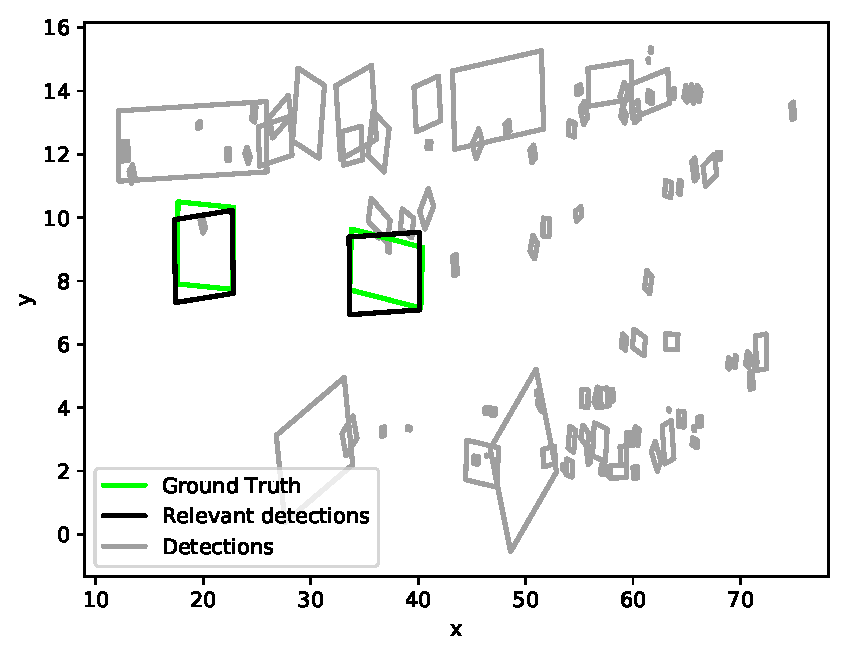
\includegraphics[width=\textwidth]{../Material/lehr2.pdf}
        \subcaption{}
        \label{fig:eval:iouLehr:2}
    \end{subfigure}
    \caption{Comparison of the estimated bounding boxes and the ground truth data, seen from above}
    \label{fig:eval:iouLehr}
\end{figure}

\section{Comparison with other algorithms}
Most of the current state of the art algorithms for object detection, such as \cite{shi2019}, 
\cite{Bin19} and \cite{Mar18}, use deep neural networks for detection and classification of the objects.
The large \ac{cnn}s used for this end-to-end detection require a lot of computational power.
\cite{Mar18} states, that Complex-YOLO runs at 50 \ac{fps} on a NVIDIA TitanX \ac{gpu}. 
As there is no official implementation publicly available, the runtime can not be measured on the vehicle.
To estimate the performance YOLO \cite{yolov3} is used, this \ac{cnn} is used for object detection on images and is the base for Complex-YOLO.
YOLO is publicly available and runs at 30 \ac{fps} on the TitanX \ac{gpu}.

Using the numbers given in Table \ref{tab:eval:yoloRuntime} the runtime of Complex-YOLO on the vehicle can be estimated, assuming that the ratio between YOLO and Complex-YOLO is independent of the device used:
\begin{equation}
    t_\text{Complex-YOLO Vehicle} \approx \frac{t_\text{Complex-YOLO TitanX}}{t_\text{YOLO TitanX}} \cdot t_\text{YOLO Vehicle} = 31s
\end{equation}

\begin{table}[h!]
    \centering
    \begin{tabular}{c|cc}
        \toprule
         & Titan X & On the vehicle\\
         \midrule
         YOLO & 33ms & 46s \\
         Complex-YOLO & 20ms & \text{approx} 31s \\ 
         \bottomrule
    \end{tabular}
    \caption{Comparison of the runtimes (Complex-YOLO on the vehicle is estimated)}
    \label{tab:eval:yoloRuntime}
\end{table}

This is only a rough approximate but the estimated time is about three magnitudes larger than the maximum time allowed. This shows that it is not possible to use a deep neural network for end-to-end detection on the vehicle without a \ac{gpu} or dedicated hardware for acceleration of the calculations.

\chapter{Conclusion} \label{sec:conc}
The objective of this work was to implement an algorithm which is able to detect and classify all objects occurring on the track of the Carolo-Cup in real time using the point cloud acquired by the \ac{d435}.

For this task an algorithm was implemented and improved to be used with point clouds acquired by stereo camera systems. 
The algorithm consists of a separate object detection and classification. 
For the detection the three dimensional space is subdivided into a two dimensional grid. 
Every cell of the grid is assigned a type, based on the number of points and the variance of the height of the points in the cell. 
All cells that belong to the foreground are clustered using connected components labeling on two scales two determine objects.
For each object an pseudo depth image is extracted and classified using a \ac{cnn}. 
Additionally a bounding box is estimated for every cluster.
To detect slopes a ground plane is estimated.

The proposed algorithm is able to robustly detect most of the required objects in the required time.
It was shown that the performance of the detector is better than the old obstacle detection, especially on the slope. 

The detection algorithm of \cite{AttBen17} was adapted for the usage with point clouds generated from stereo data. The proposed changes have improved the overall performance of the algorithm when compared with both the original algorithm on stereo and Lidar data.

Furthermore the algorithm has been evaluated on data acquired with stereo systems in the real world. 
With this data the performance depends on the quality of the point cloud. 
As a result of the small baseline distance of the camera system of the Kitti dataset the quality of the point cloud is only sufficient for a distance of up to ten meters.
Due to the larger baseline of the system in Ulm-Lehr the quality of the point cloud is much better, for this data the algorithm is able to detect objects at a distance of over $50\si{\m}$.

\section{Future improvements}
The performance of the algorithm depends on the quality of the point cloud, thus a better point cloud improves the quality of the detections. 
The quality of the point cloud can be improved by using a better stereo matching algorithm, such as \cite{chang2018pyramid} \cite{luo16} \cite{zbontar16}. 
They perform stereo matching using \ac{cnn}s, this improves the quality of the point cloud but requires a lot of processing time. 
Thus it is not a viable option for the Carolo-Cup, but for the real world data it can improve the quality of the point clouds.

To make the detection less prone to the varying quality of the point cloud the classification of the cell needs to be improved. For this an \ac{mlp} which classifies the histogram over the $z$ values of all points in a cell could be used. Such a neural network would run sufficiently fast, even without a \ac{gpu}, but due to limitations in time this approach has not been pursued.


\appendix

\backmatter

\printbibliography

\clearpage
\thispagestyle{empty}

Name: \fullname \hfill Matrikelnummer: \matnr \vspace{2cm}

\minisec{Erklärung}

Ich erkläre, dass ich die Arbeit selbständig verfasst und keine anderen als die angegebenen Quellen und Hilfsmittel verwendet habe.\vspace{2cm}

Ulm, den \dotfill

\hspace{10cm} {\footnotesize \fullname}
\end{document}
